% ============================================================
%  EdgeBench 中文翻译 —— 正文(第1--7章)
%  原文: arXiv:2607.15651v1, ByteDance Seed, 2026-07-07
% ============================================================

% ============================================================
\section{引言}
\label{sec:intro}

预训练阶段的缩放规律~\cite{kaplan2020,hoffmann2022}揭示了模型能力可随数据量与算力的增加而\textbf{可预测地}提升。这一洞见指导了过去数年大语言模型领域的诸多重要进展~\cite{anthropic2024claude,dubey2024llama3,openai2023gpt4,openai2025gpt45,openai2025gpt5,openai2025gpt52,openai2025gpt5sc,gemini2024gemini15,gemini2025gemini25}。如今,大语言模型正迈入``智能体(Agent)时代'',它们被部署到日益多样的真实世界环境中,能够在交互中尝试学习。然而,这种``从环境中学习''是否同样服从简洁的缩放规律,迄今仍属未知。

通过对\textbf{134}个真实世界任务上累计约 \textbf{38{,}000} 小时的智能体环境交互数据进行分析,我们(据我们所知)首次发现了\textbf{环境学习整体性能随交互时间遵循对数-S 形(log-sigmoid)缩放规律}这一证据,且拟合精度极高,$R^2 = 0.998$。

\begin{figure}[h]
\centering
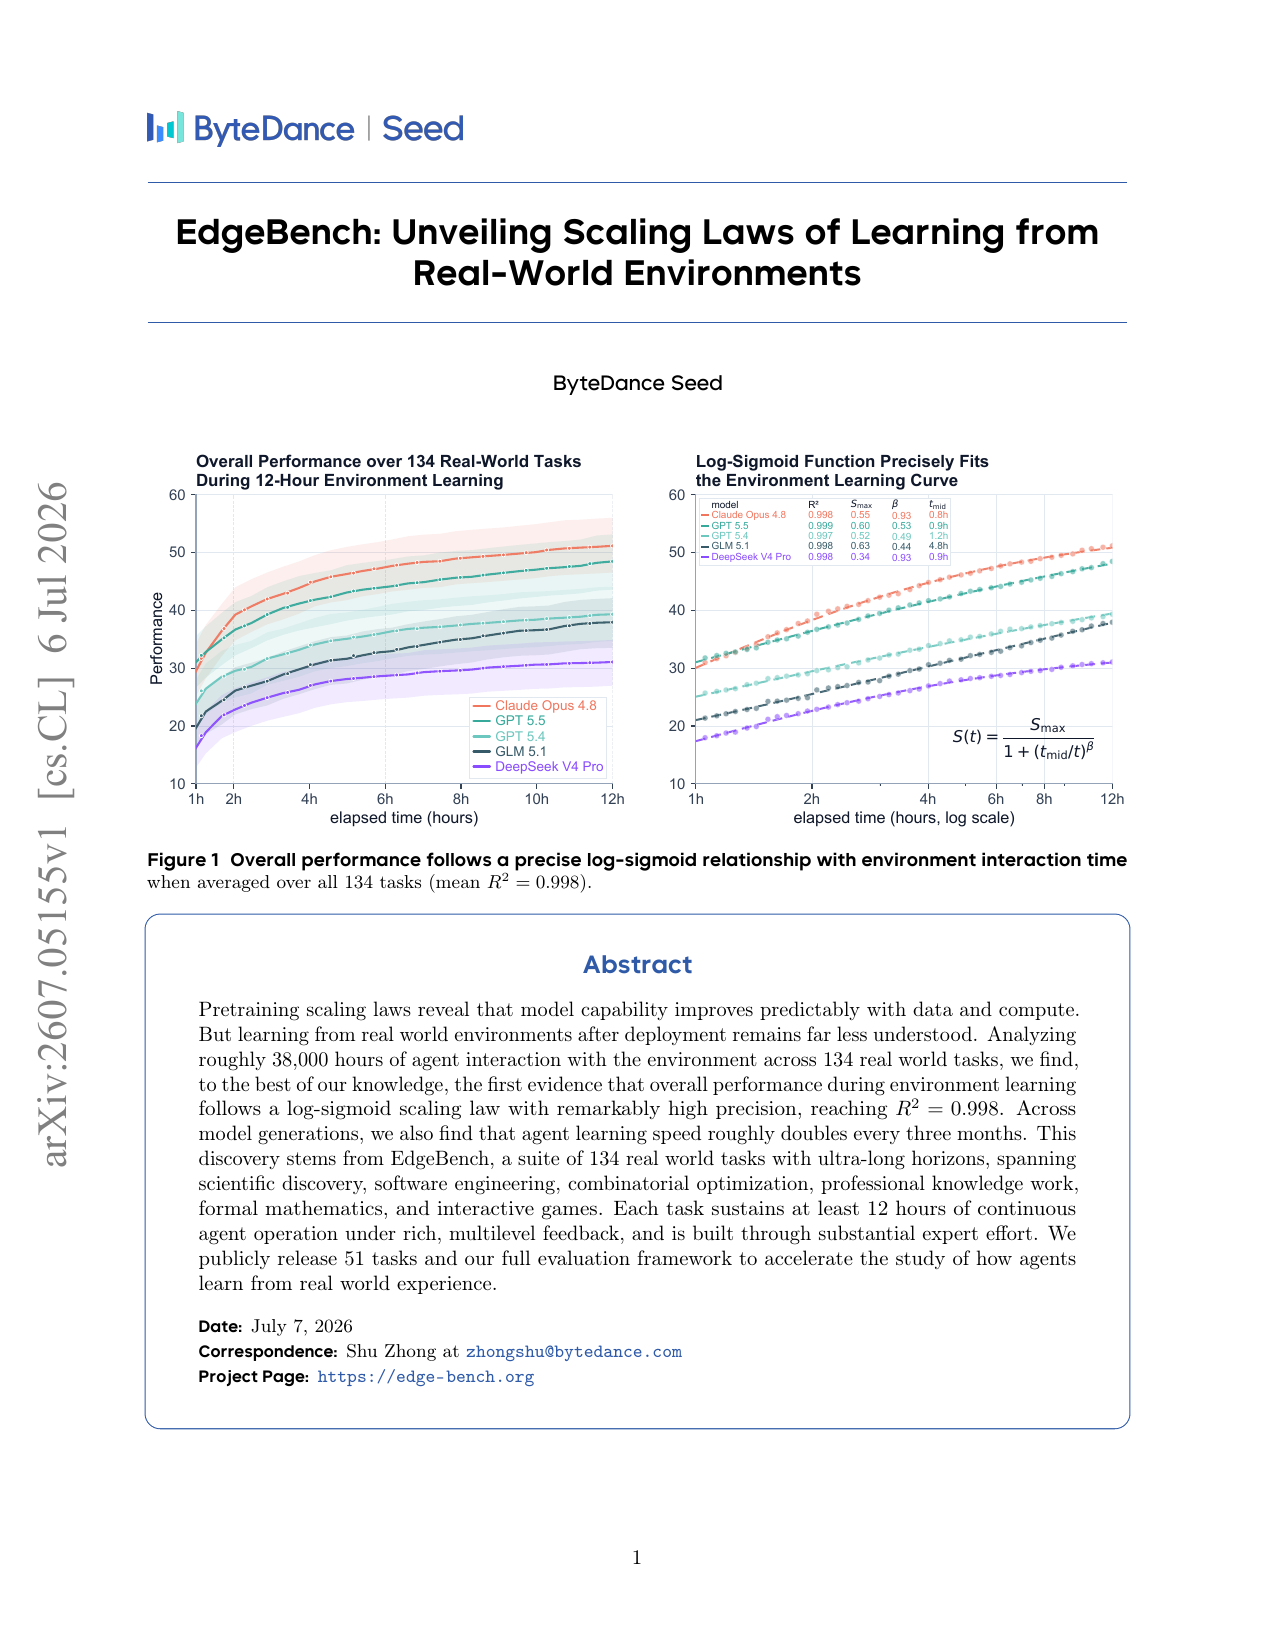
\includegraphics[width=0.95\textwidth]{figures/page-01.png}
\caption{整体性能随交互时间呈现精确的对数-S 形关系($134$ 个真实世界任务求均值,$R^2 = 0.998$)。}
\label{fig:overview}
\end{figure}

\paragraph{为什么研究智能体从环境中学习的能力?}
真实世界的 AI 应用远不止模型在训练阶段学到的那些能力。一些必要知识从未出现在训练数据中——例如私有记录和内部工具。即便原始数据存在,也往往缺失了背后的人类过程:反复试错、对证据的解读、依据反馈做出的适应性调整——而这正是专家实际取得成果的方式。真实世界也从未静止:人类知识持续前进,新的工具、发现与问题不断涌现,任何固定的训练语料都无法预见。因此,智能体从环境中学习并提升任务表现的能力,是 AI 系统大规模部署到真实世界的核心要素。

研究这种能力需要任务环境具备以下三个条件:(1) 接近真实使用场景;(2) 提供富有信息量的学习反馈;(3) 允许智能体通过交互进行足够长时间的学习。然而,现有的评测基准要么缺乏这种反馈,要么把智能体的运行时间限定为几分钟到几小时~\cite{chan2025mle,jimenez2024swebench,merrill2026terminalbench,sun2026agents,xu2026autolab,wei2025browsecomp},因此并不适合本研究的目标。为弥补这一空白,我们构建了 \textbf{EdgeBench}:一个由 134 个真实、多样化任务组成的评测套件,横跨六个能力家族(参见图~\ref{fig:taxonomy})。每个任务运行在一个可执行的工作区中,结合快速的本地探索与较慢的、针对提交产物的判官反馈,以模拟真实工作流。智能体可在每个任务上持续工作\textbf{至少 12 小时}(相比之下,Agents' Last Exam~\cite{sun2026agents} 平均每个任务仅约 1 小时);同时,我们记录其提交并追踪表现随时间的演进。这些任务对人类专家而言也极具挑战性:记录的专家投入平均为 \textbf{57.2 小时/任务},最高达 \textbf{320 小时/任务}。这使 EdgeBench 自然成为研究智能体如何\textbf{在长视野下}从环境中学习的理想测试平台。

借助 EdgeBench,我们在约 \textbf{38{,}000 小时}的环境交互上评测了前沿智能体,并归纳出\textbf{四项核心观察}:

\begin{enumerate}
    \item \textbf{环境学习呈现出精确的对数-S 形缩放规律}——在跨任务求平均的总体曲线、各任务家族、更长至 72 小时的交互视野下,以及在用早期轨迹预测后期性能时,均呈现相同函数形式;
    \item \textbf{对数-S 形规律的理论推导}——我们提出一种理论,将环境学习建模为在潜在任务图(latent task graph)上的``前沿扩张(frontier expansion)''过程,从而解释了为何基准求平均后的进度呈现观察到的对数-S 形;
    \item \textbf{智能体学习速度大约每三个月翻倍}——研究自 2025 年 9 月以来发布的前沿模型,即可发现前沿智能体的环境学习速度正快速提升;
    \item \textbf{学习动力学强烈影响长视野表现}——长视野性能取决于智能体如何利用已积累的经验,而不仅仅是尝试了多少次。连续使用经验优于独立重启,更长上下文提升记忆能力,而详尽的案例研究表明:反馈能够将大量失败的试探转化为少数持久性的进展。
\end{enumerate}

% ============================================================
\section{EdgeBench}
\label{sec:bench}

\subsection{设计目标}
\label{sec:design}

EdgeBench 的目标是衡量一个自主智能体能否在陌生的真实世界环境中\textbf{通过经验学习}。这对评测基准提出了两项现有评估无法满足的要求:

\begin{itemize}
    \item \textbf{超长视野、多样化任务。} 探索、策略修订、经验积累等学习行为需要足够的时间和复杂度才能显现。短任务通常依赖记忆而非学习来求解,因此要衡量学习能力就必须使用长视野任务。此外,学习是一种通用能力,这些任务还需横跨多样化领域。
    \item \textbf{真实、多层次的反馈。} 在实践中,人类专家从丰富反馈中学习:测试失败、实验结果、反常现象、权威判断等等。无法提供如此丰富反馈的基准,既无法衡量学习,也会让智能体无从知晓评测究竟奖励什么。我们需要近似真实世界的反馈,才能衡量真正的、通用目的的学习能力。
\end{itemize}

第一项要求驱动了我们的任务分类体系(详见 \secref{sec:taxonomy}):跨六个能力家族共 134 个任务,每个任务都被设计为至少 \textbf{12 小时} 量级、可承受前沿模型运行的挑战。第二项要求驱动了我们的评测协议(详见 \secref{sec:protocol}):每个任务独立模拟其专属的``真实世界''切片,提供\textbf{隔离的工作环境与判官环境}、本地智能体驱动的反馈、提交门控的判官反馈以及宿主端的轨迹测量。

\subsection{任务分类体系}
\label{sec:taxonomy}

我们搜索满足两条标准的真实任务:(1) 性能上限足够高,使任何现有智能体都无法将其饱和;(2) 工作流支持\textbf{连续学习}而非一次性完成。这一搜索与跨领域专家协作进行,共识别出六个能力家族、产出 134 个精心挑选的任务(图~\ref{fig:taxonomy}):

\begin{figure}[h]
\centering
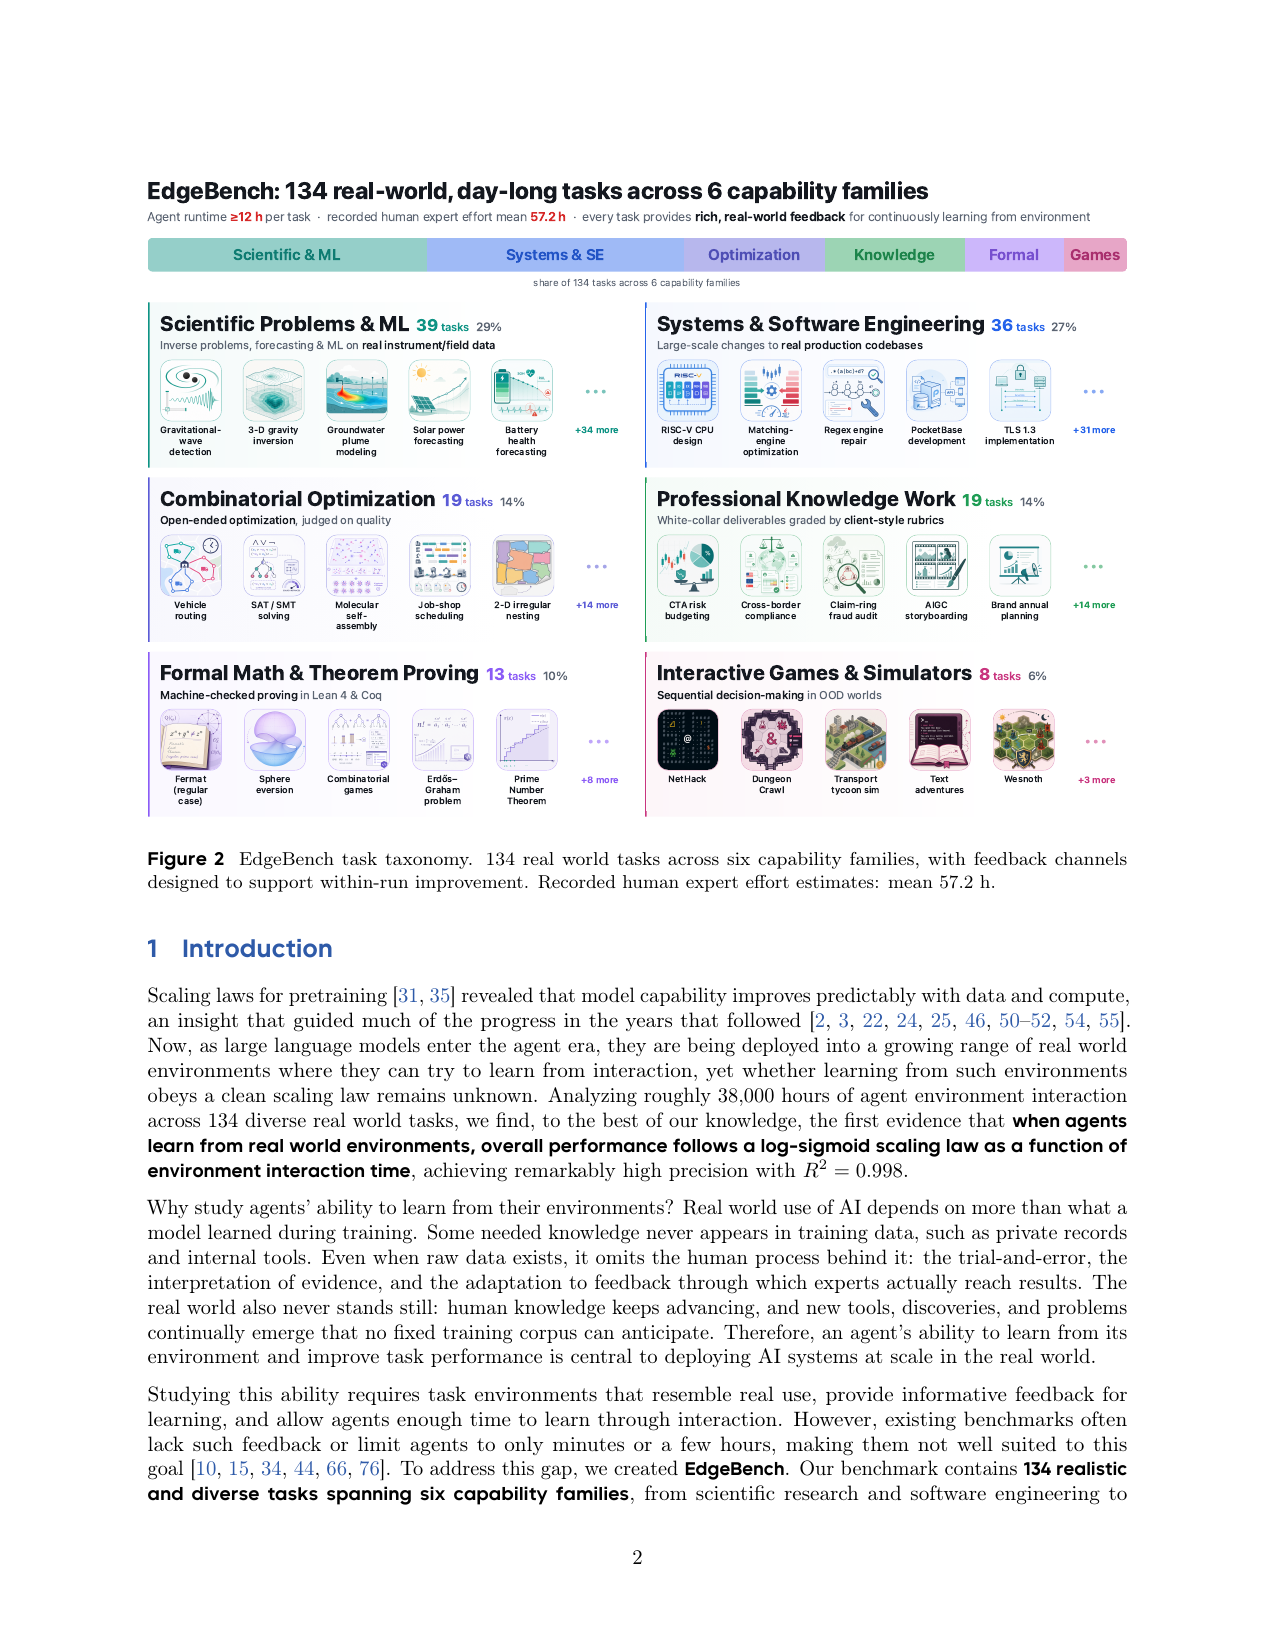
\includegraphics[width=0.95\textwidth]{figures/page-02.png}
\caption{EdgeBench 任务分类。134 个真实任务横跨六个能力家族,每个家族均设计了支持 ``run 内改进'' 的反馈通道。记录的人工专家投入均值 57.2 小时/任务。}
\label{fig:taxonomy}
\end{figure}

\begin{itemize}
    \item \textbf{科学问题与机器学习(Scientific Problems \& ML,39 个任务)}。每个任务均使用来自真实科研工作者的研究数据与实验设置。领域专长不可或缺:智能体必须提出假设、选择模型、在有噪声观测上验证、并迭代优化。许多问题是开放式的,尚无已知最优解。
    \item \textbf{系统与软件工程(Systems \& Software Engineering,36 个任务)}。智能体在生产级代码库上工作,单个任务可能需要数千行代码改动,在最大的案例中涉及超过 10 万行。由于代码跨模块相互依赖,智能体必须同时考虑跨模块耦合以及正确性与性能目标。
    \item \textbf{组合优化(Combinatorial Optimization,19 个任务)}。这些开放式、以 NP-hard 问题为主的任务中,精确方法不可行,进度依赖于设计、调参与迭代启发式搜索策略。即使强大的求解器也有在更多时间与反馈下提升的空间。
    \item \textbf{专业知识工作(Professional Knowledge Work,19 个任务)}。这些任务复现金融、教育、医疗、法律等领域的真实白领交付物——通常需要三年以上经验的从业者约三个完整工作日才能完成。许多任务具备精心设计的评分细则和多轮交付反馈,以近似真实客户审阅循环,使智能体可从结构化批评中学习并迭代修订。
    \item \textbf{形式化数学与定理证明(Formal Math \& Theorem Proving,13 个任务)}。这些任务位于数学难度的前沿,需要在 Lean 中构建大规模机器可检查证明,将深邃的数学洞察与大量形式化验证工程相结合。大部分任务为 EdgeBench 全新设计,以支持迭代进展:智能体获得结构化的中间指引,并可增量扩展局部证明。
    \item \textbf{交互式游戏与模拟器(Interactive Games \& Simulators,8 个任务)}。这些是为人类玩家设计的真实游戏,熟练的人类通常需要数十小时才能掌握机制。状态空间极大且每局游戏程序化地不同,因此智能体面临强大的\textbf{分布外(Out-of-Distribution, OOD)}压力,必须通过跨多个episode的高频交互开发并优化策略。
\end{itemize}

\textbf{任务排除说明}:主要难度来自视觉理解(尤其是 GUI 操作)的任务被排除。当成功取决于视觉骨干而非迭代推理时,学习能力与感知能力难以分离。

% ============================================================
\subsection{反馈循环与评测协议}
\label{sec:protocol}

真实世界的工程与研究工作流很少提供单一的``最终答案''检验。实际上,从业者通过\textbf{两条互补的反馈循环}迭代:一条用于探索、调试与精炼的\textbf{快速本地循环},以及一条通过部署、同行评审、基准评测或干系人反馈进行权威校准的\textbf{较慢外部循环}。本地循环促成快速进展,外部循环防止对可见检验的过拟合,并揭示开发者自身测试未覆盖的失败。

\begin{figure}[h]
\centering
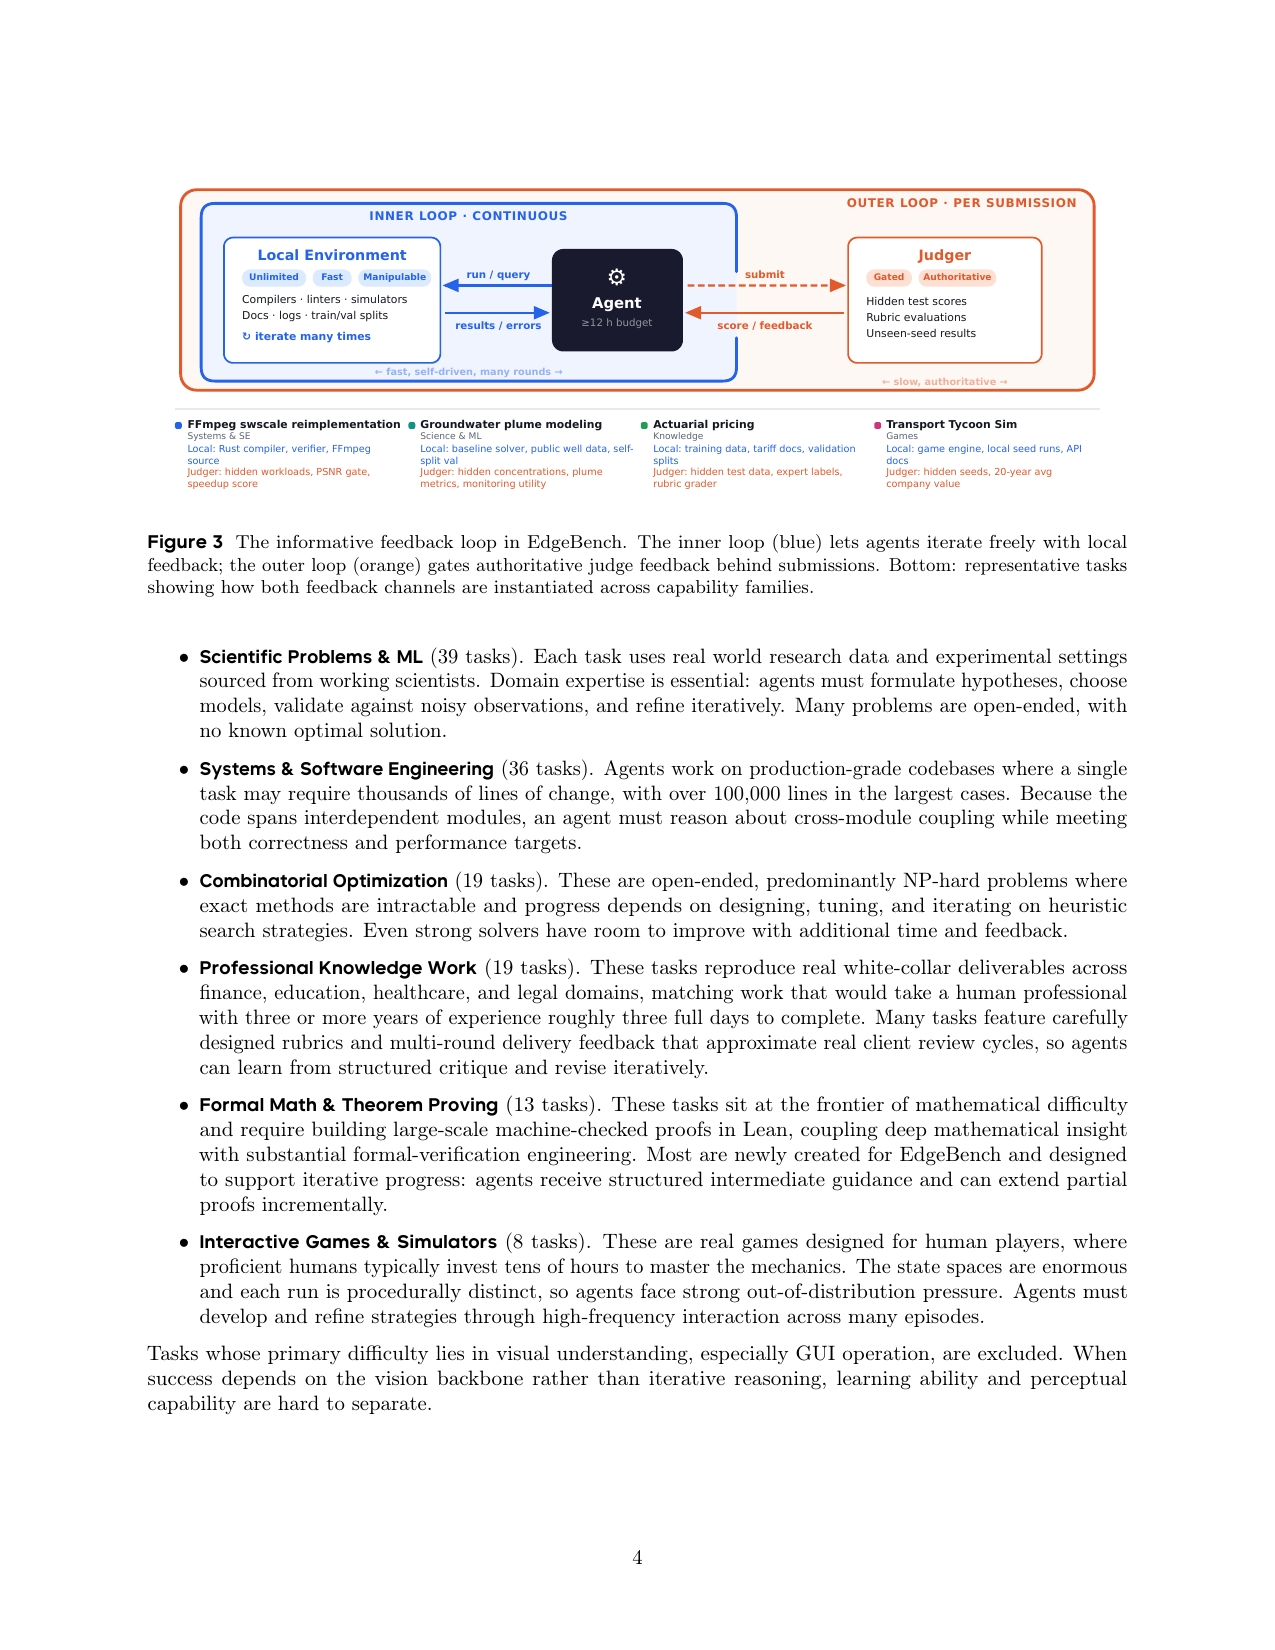
\includegraphics[width=0.95\textwidth]{figures/page-04.png}
\caption{EdgeBench 的信息反馈循环。内循环(蓝色)允许智能体基于本地反馈自由迭代;外循环(橙色)将权威判官反馈置于提交门控之后。下方展示了六大家族中该反馈模式的具体实例化。}
\label{fig:feedback}
\end{figure}

EdgeBench 采用这种``双循环''结构来衡量学习而非端点成功(参见 \figref{fig:feedback})。内循环是本地且由智能体驱动:智能体可检视可写工作区、运行测试或模拟器、观察错误、修订产物。外循环由判官中介:提交的产物将基于隐藏用例或私有评分标准进行评估,返回校准后的分数、判定或诊断。跨任务家族,这一模式通过不同机制实例化:软件任务使用测试与性能分析器,科学任务使用开发拆分与验证器,优化任务使用本地测试器与隐藏随机种子,定理证明使用证明检查器的状态,游戏使用 episode 分数,专业知识工作使用评分细则。

该协议由一个\textbf{隔离的工作—判官评测沙箱}实现。在运行期间,智能体在一个容纳任务材料与本地验证工具(但不包含隐藏评测资产)的\textbf{工作容器(Work Container)}内工作。智能体可主动将其当前产物提交到一个独立的\textbf{判官容器(Judge Container)},该容器运行隐藏评测并返回任务定义的反馈。宿主端的判官服务器负责中介这一外循环,包括提交队列、冷却时间、身份认证以及支持长时评测的异步评分,使智能体在提交作业评分的同时继续工作。附录~\ref{app:hacking} 给出了一些促使我们采用隔离与提交中介设计的失败模式示例。

为进行轨迹测量,评测沙箱还会按固定间隔执行宿主端自动评测。这些快照通过隐藏判官评分并被记录用于分析,但\textbf{结果不会展示给智能体}。这使得 EdgeBench 即便在两次显式提交之间也能衡量改进,同时保留了``智能体可见反馈''与``评测者专属测量''之间的区分。

% ============================================================
\section{真实世界环境学习的缩放规律}
\label{sec:scaling}

经典预训练缩放规律~\cite{kaplan2020,hoffmann2022}将语言模型损失建模为训练规模的幂律函数,包括预训练数据量~\cite{kaplan2020,hoffmann2022}。相比之下,基准性能则是模型能力的``任务级''读数,受任务、样本与评分标准引入的难度阈值所塑造。先前的工作~\cite{bhagia2024ladder,owen2024predictable,ruan2024observational,zhang2026prescriptive}发现,在预训练规模扩展下,基准性能可用对数-S 形曲线良好描述。

除了从人类收集的训练数据中学习,现代智能体(如 GPT-5.5~\cite{openai2026gpt55}、Claude Opus 4.8~\cite{anthropic2026opus48})还可在部署后继续从环境中学习。在单个任务上,它们可以通过交互获取新信息并随时间提升性能。然而,这种学习形式是否同样服从简洁的缩放规律,仍不清晰。EdgeBench 提供了 134 个多样化的真实世界任务,具备可执行环境、富有信息量的反馈以及至少 12 小时的交互视野,使我们得以研究智能体如何通过与环境交互提升性能。通过在 134 个多样化真实任务上分析五个前沿智能体约 \textbf{38{,}000 小时}的环境交互,我们发现\textbf{对数-S 形曲线能够精确拟合环境学习性能}。因此,环境学习与预训练数据学习诱导出了\textbf{相同的数学缩放形式}。

\subsection{从任务轨迹到可预测的缩放曲线}
\label{sec:exp-setup}

\paragraph{实验设置。} 我们用五个前沿模型评估 134 个 EdgeBench 任务:Claude Opus 4.8~\cite{anthropic2026opus48}、GPT-5.5~\cite{openai2026gpt55}、GPT-5.4~\cite{openai2026gpt54}、GLM-5.1~\cite{zai2026glm51,glm52026} 以及 DeepSeek-V4-Pro(preview)~\cite{deepseek2026v4}。每个``任务-模型''配对运行三次独立的 12 小时试验,并记录完整提交轨迹。GPT 系列模型使用 Codex 与 256k 紧凑上下文窗口运行;GLM-5.1 与 DeepSeek-V4-Pro 使用 Claude Code 与 200k 紧凑窗口运行。Claude Opus 4.8 主要使用 1M Claude Code 紧凑窗口运行;此外我们在 \secref{sec:ctx} 中加入了一个 200k vs.\ 1M Opus 消融实验。

\paragraph{逐任务轨迹的多样性。} 图~\ref{fig:per-task-curves} 展示了 18 个代表性任务的逐任务学习曲线,展示了不同模型如何在同一任务上随时间改进。所有任务的完整曲线集合见附录~\ref{app:per-task-curves}。任务横跨多样化领域,表现出异构的学习动力学:轨迹范围从平滑渐进增益到长平台、突变突破乃至不规则回退。

\begin{figure}[h]
\centering
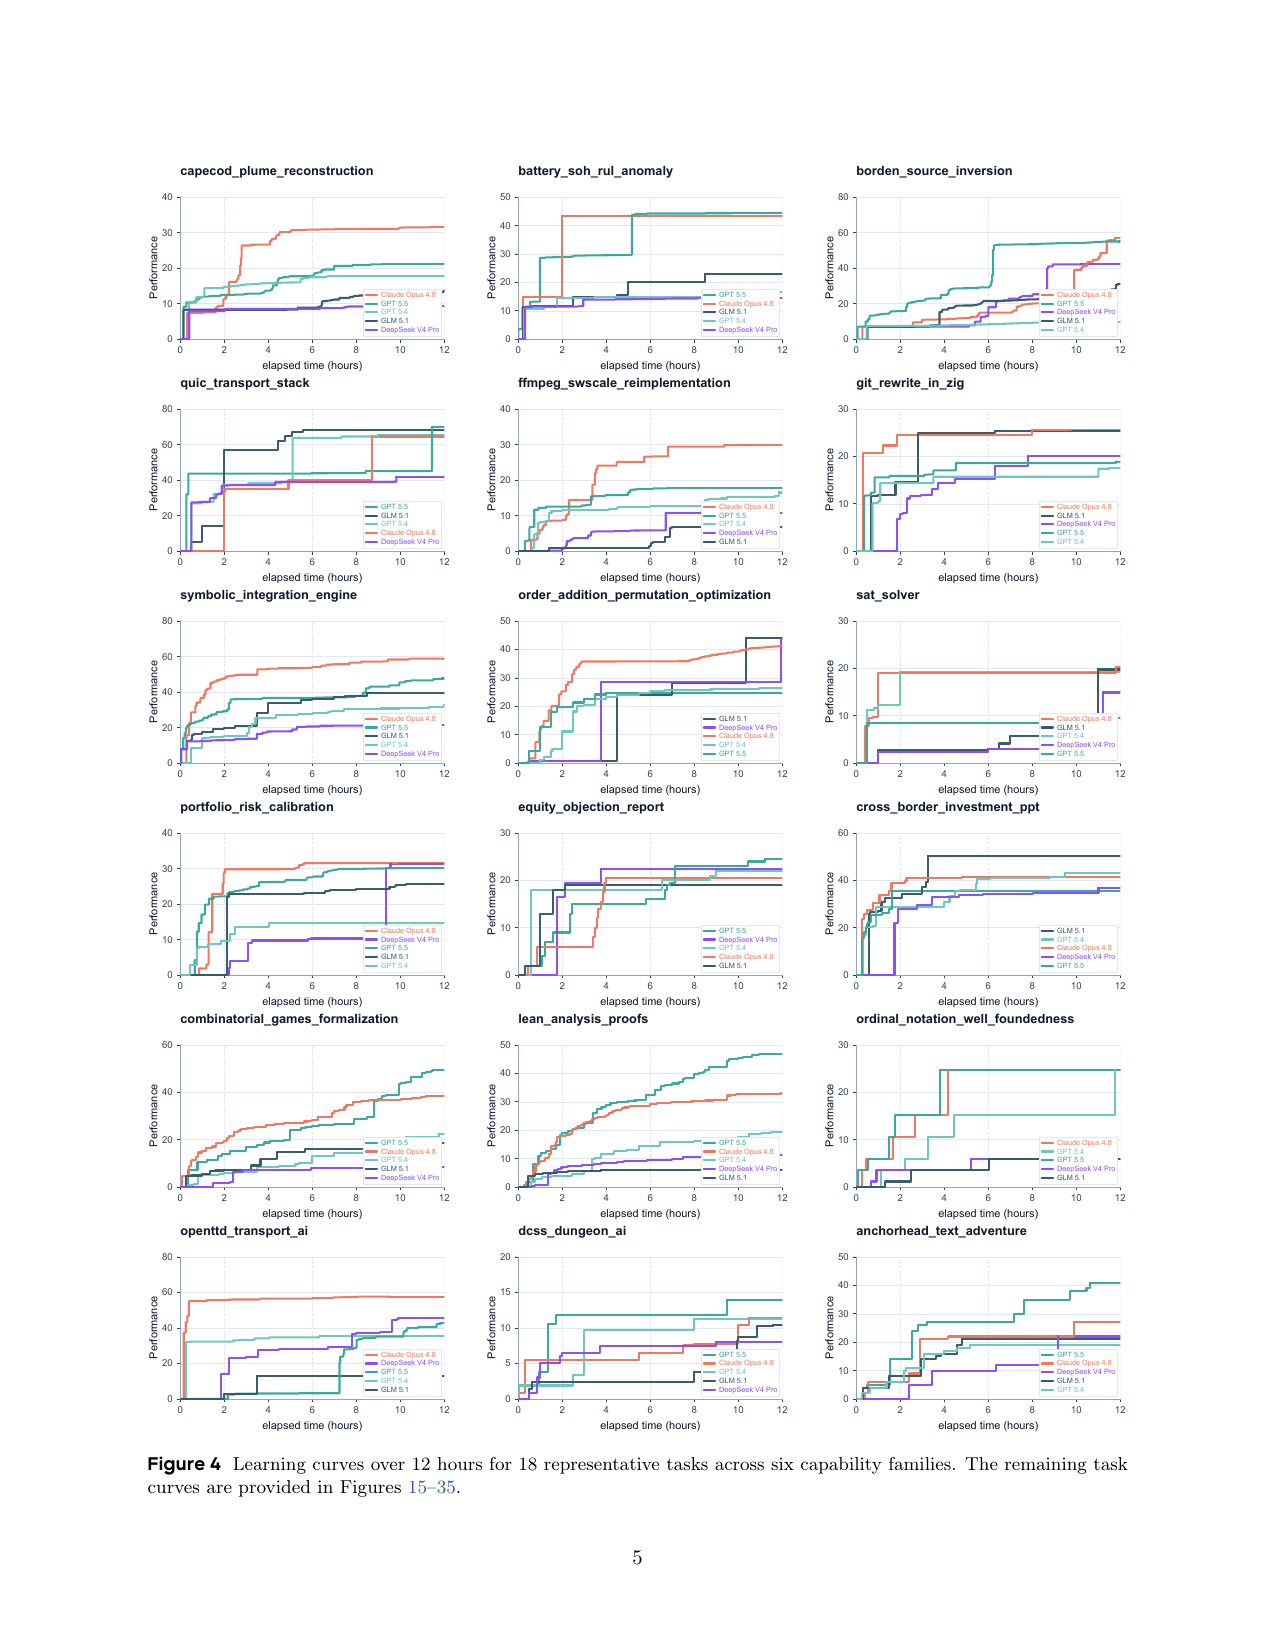
\includegraphics[width=0.95\textwidth]{figures/page-05.png}
\caption{18 个代表性任务跨 12 小时的学习曲线,涵盖六个能力家族。其余任务曲线见附录图~\ref{app:per-task-curves}。}
\label{fig:per-task-curves}
\end{figure}

\paragraph{聚合曲线揭示共同结构。} 虽然这些个体曲线在任务与模型间高度异质,但其跨任务平均曲线却出乎意料地\textbf{平滑}且具有共同结构。受先前在预训练扩展下对对数-S 形基准拟合的启发~\cite{bhagia2024ladder,owen2024predictable,ruan2024observational},我们用以下\textbf{三参数对数-S 形}模型拟合平均后的环境学习曲线:

\begin{equation}
    S(t) = \frac{S_{\max}}{1 + (t_{\mathrm{mid}}/t)^{\beta}},
    \label{eq:log-sigmoid}
\end{equation}

其中 $t$ 为已用交互时间,$S(t)$ 为\textbf{迄今最佳性能(best-so-far performance)}。拟合参数作为聚合学习曲线的经验性描述符:
\begin{itemize}
    \item $S_{\max}$ —— 可达到的分数上限;
    \item $t_{\mathrm{mid}}$ —— 曲线达到该上限一半时所对应的交互时间;
    \item $\beta$ —— 控制在对数时间下进度集中的陡峭程度。
\end{itemize}
因此,较小的 $t_{\mathrm{mid}}$ 意味着模型更快达到可达到分数的主体部分;较大的 $\beta$ 对应更陡的学习跃迁。\secref{sec:fit-quality} 显示这种简洁函数形式能极其精确地拟合经验学习曲线。

% ============================================================
\subsection{对数-S 形曲线以惊人精度拟合环境学习}
\label{sec:fit-quality}

我们发现对数-S 形拟合在所有测试设置下都精确且稳健:

\begin{enumerate}
    \item \textbf{对数-S 形曲线精确拟合 134 任务的平均值,适用于所有五个模型。} 如 \figref{fig:overview} 所示,在对 134 个任务求平均后,拟合的对数-S 形曲线紧密跟踪每个模型的 12 小时学习轨迹。拟合在所有五个模型上都相当紧密,$R^2 \geq 0.997$。
    \item \textbf{相同的对数-S 形形式在异构的任务家族间持续成立。} \figref{fig:family} 重复地对 EdgeBench 中六个能力家族分别进行拟合。这些家族需要不同的知识、锻炼不同的能力,且呈现明显不同的聚合学习曲线。然而,每个家族仍可被相同的对数-S 形形式良好描述——即使在任务数较少、均值轨迹噪声较大的小型家族中也成立。
    \item \textbf{在显著更长的交互视野下拟合仍然精确。} \figref{fig:long-horizon} 将分析扩展到主 12 小时窗口之外,达到 28 小时与 72 小时的交互视野。受资源所限,28 小时拟合覆盖 80 个任务与四个模型,72 小时拟合覆盖 18 个任务与两个模型。相同的对数-S 形结构在两种更长设置下保持稳定,每条拟合曲线均达到 $R^2 \geq 0.993$。
    \item \textbf{对数-S 形规律展现预测能力。} \figref{fig:forecast-and-long} 通过仅用前 6.5 小时拟合每条 12 小时聚合曲线来验证这一预测能力,然后在 6.5--12 小时的\textbf{留出观测}上评估外推。所有五个模型下,外推曲线仍贴近后期的观测轨迹,$R^2 \geq 0.997$、RMSE 小于 1.0 性能点。
\end{enumerate}

\begin{figure}[h]
\centering
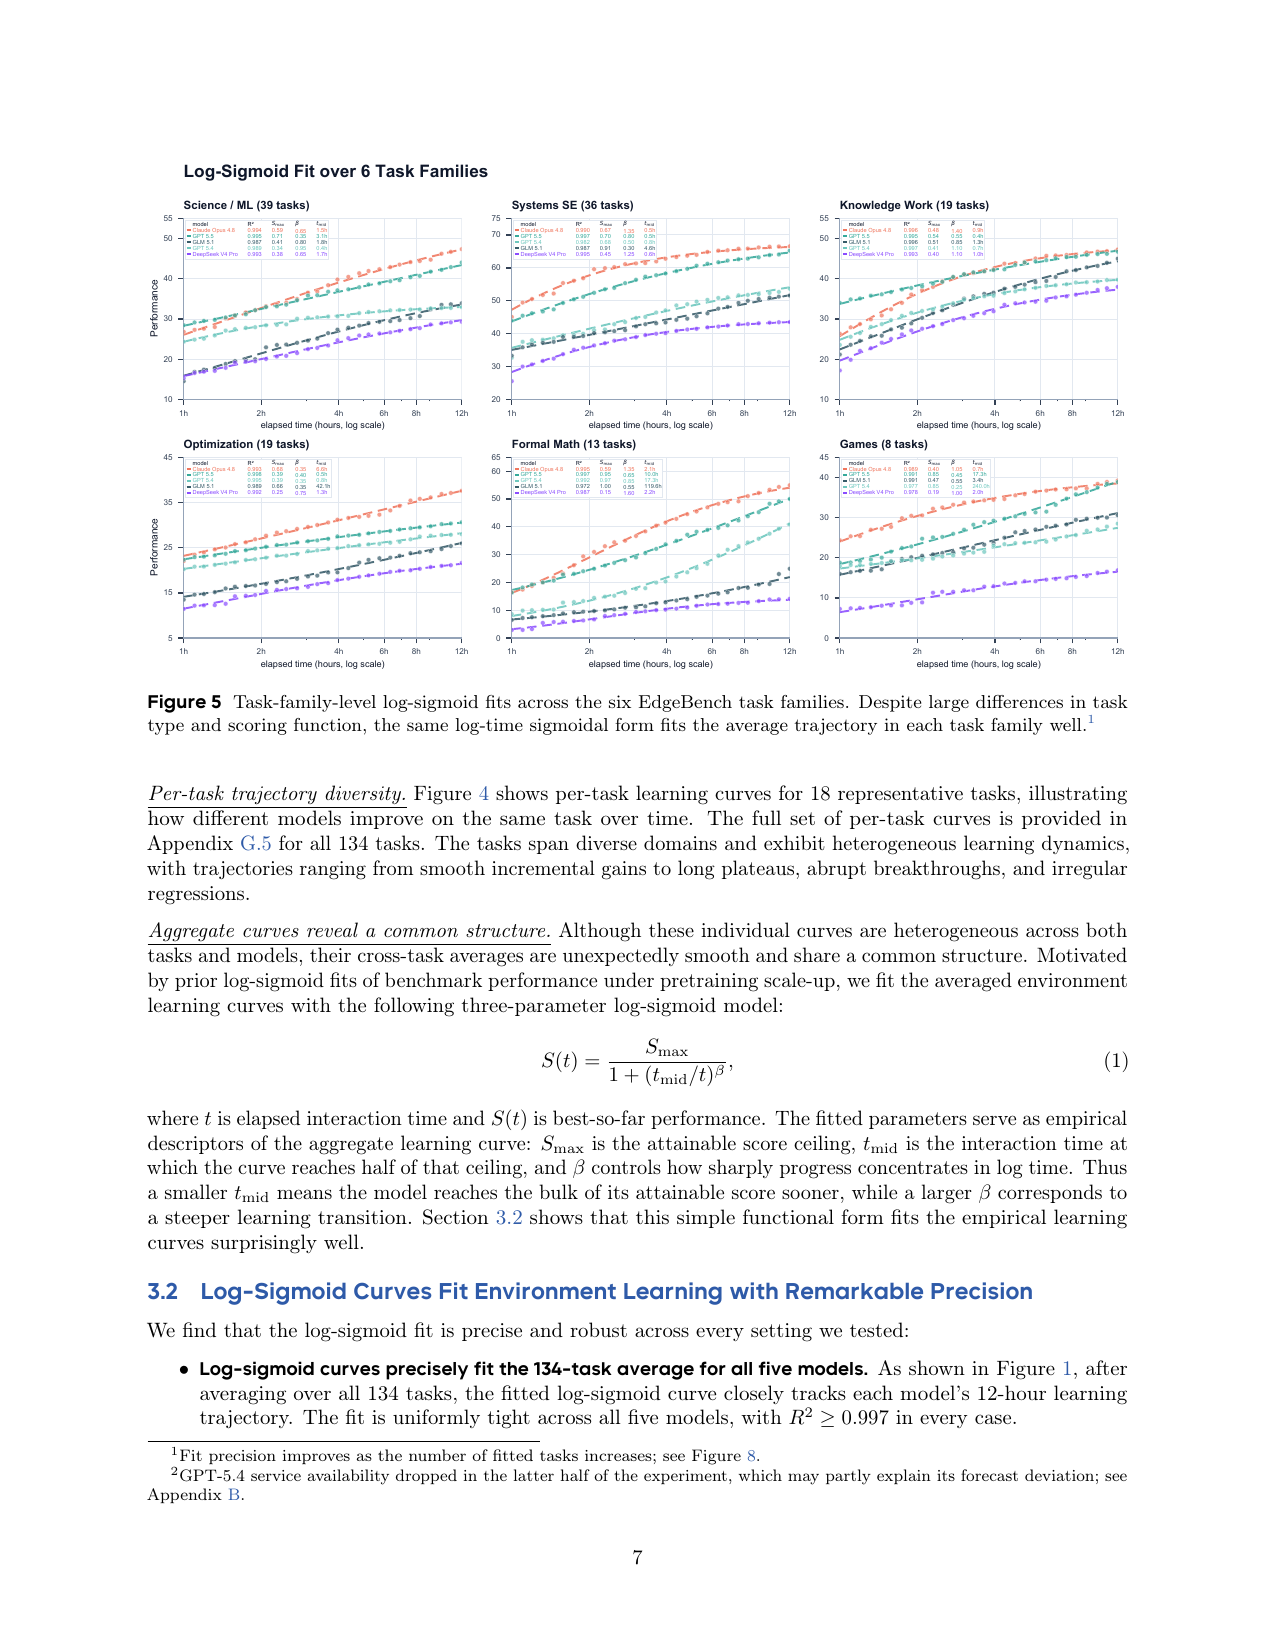
\includegraphics[width=0.95\textwidth]{figures/page-07.png}
\caption{EdgeBench 六个任务家族的逐家族对数-S 形拟合。尽管任务类型与评分函数差异巨大,同一对数时间下的 S 形形式仍能良好拟合每个家族的均值轨迹。}
\label{fig:family}
\end{figure}

\begin{figure}[h]
\centering
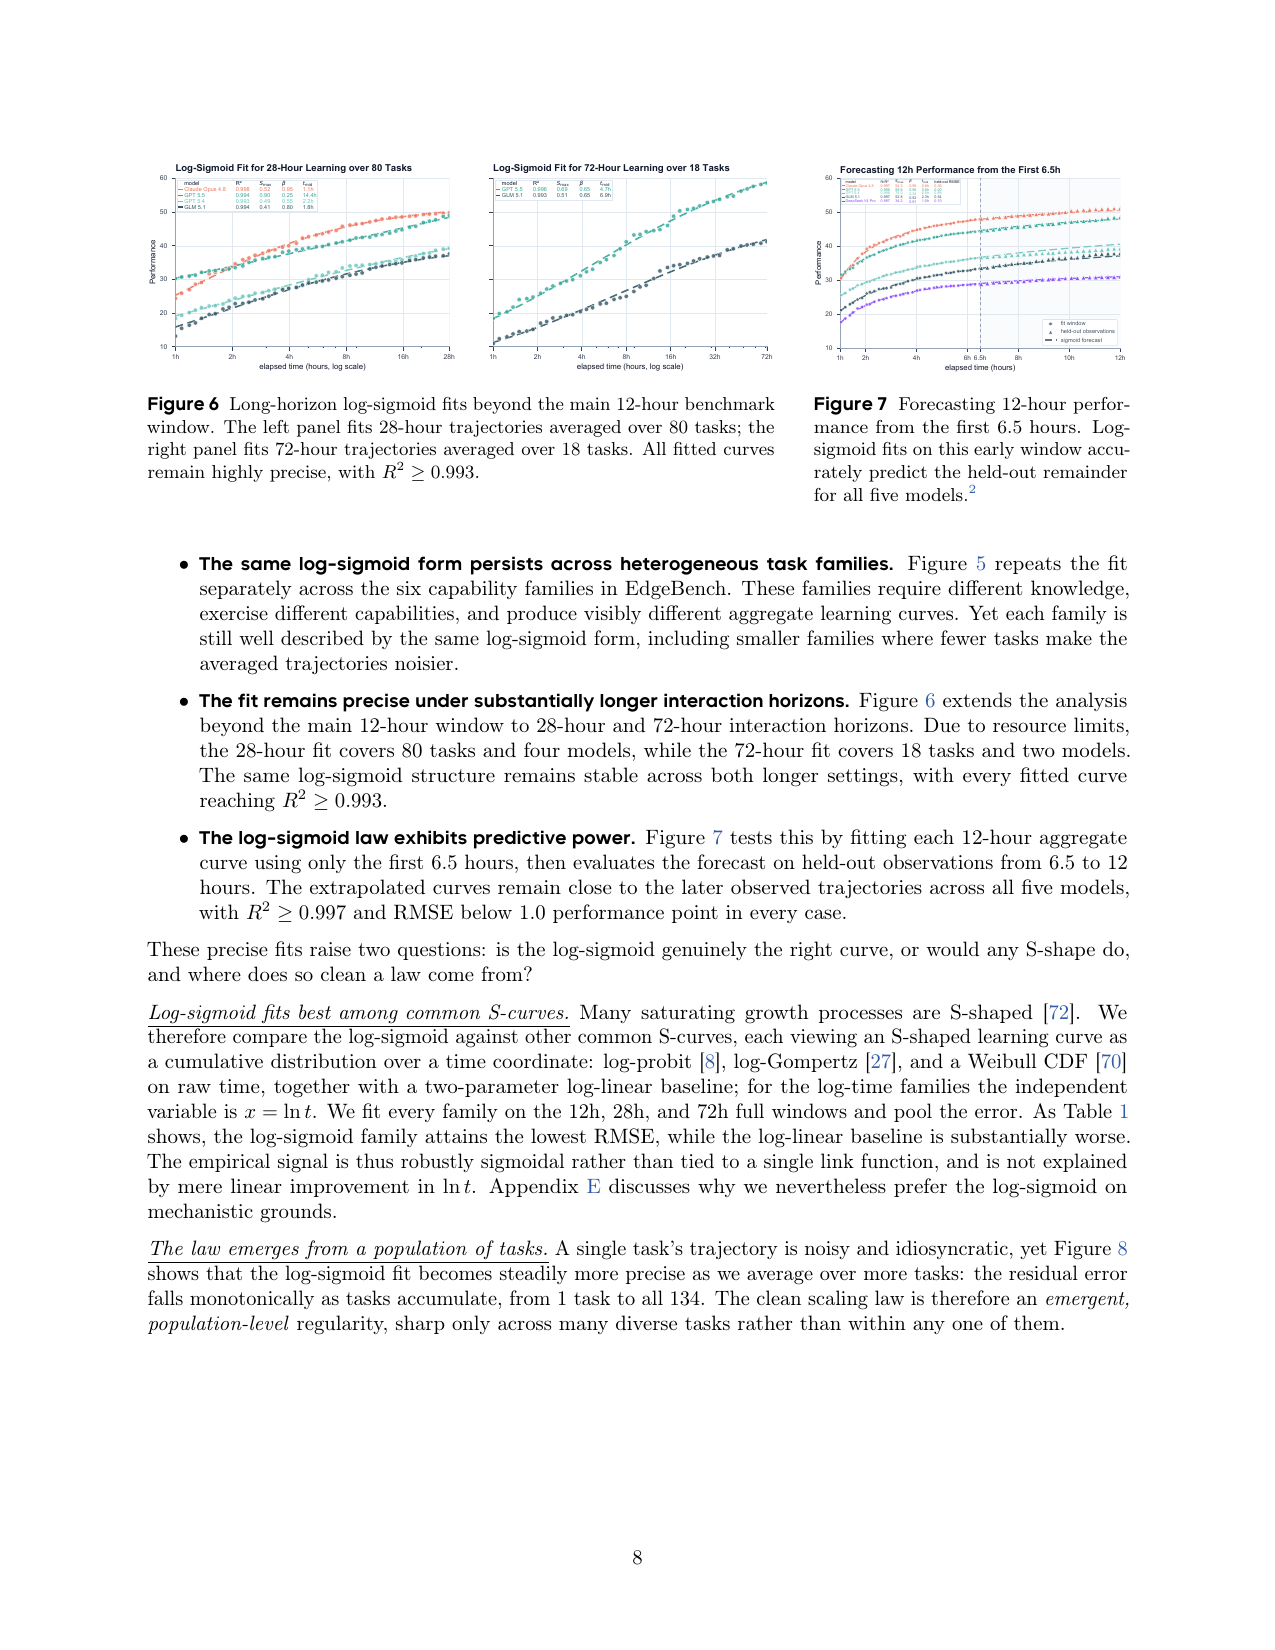
\includegraphics[width=0.95\textwidth]{figures/page-08.png}
\caption{用前 6.5 小时预测 12 小时性能以及超长视野拟合。\textbf{左图} 对 80 个任务的 28 小时轨迹取平均拟合;\textbf{右图} 对 18 个任务的 72 小时轨迹取平均拟合。所有拟合曲线仍非常精确,$R^2 \geq 0.993$。}
\label{fig:forecast-and-long}
\end{figure}

这些精确拟合引出两个问题:对数-S 形真的就是``对的''曲线吗?还是任意 S 形都行?如此简洁的规律究竟从何而来?

\paragraph{对数-S 形在常见 S 形曲线中拟合最佳。} 许多饱和增长过程都是 S 形的~\cite{wikipedia2025sigmoid}。因此我们将对数-S 形与其他常见 S 形比较:对数-Probit~\cite{bliss1934probits}、对数-Gompertz~\cite{gompertz1825} 和基于原始时间的 Weibull 累积分布函数(CDF)~\cite{weibull1951} 以及一个两参数对数-线性基线;对基于对数时间的曲线族,自变量设为 $x = \ln t$。我们对 12h、28h、72h 全窗口拟合每一族并汇总误差。如表~\ref{tab:s-curves} 所示,对数-S 形族取得最低 RMSE,而对数-线性基线显著较差。因此经验信号稳健地呈 S 形而非依赖于单一连接函数,也不能仅由对 $\ln t$ 的线性改进解释。附录~\ref{app:shapes} 从机制层面进一步论证我们为何仍偏好对数-S 形。

\begin{table}[h]
\centering
\small
\begin{tabular}{lll}
\toprule
\textbf{曲线族} & \textbf{函数形式} & \textbf{RMSE} \\
\midrule
对数-S 形 & $S(t) = \dfrac{S_{\max}}{1 + (t_{\mathrm{mid}}/t)^{\beta}}$ & \textbf{0.390} \\
对数-Probit & $S(t) = S_{\max}\, \Phi\!\left(\dfrac{\ln t - \mu}{\sigma}\right)$ & 0.398 \\
对数-Gompertz & $S(t) = S_{\max}\,\exp\!\left[-\exp\!\left\{-c(\ln t - x_{0})\right\}\right]$ & 0.402 \\
Weibull CDF & $S(t) = S_{\max}\!\left(1 - \exp\{-(t/\lambda)^{\beta}\}\right)$ & 0.404 \\
对数-线性 & $S(t) = a + b\ln t$ & 0.717 \\
\bottomrule
\end{tabular}
\caption{三参数 S 形族与两参数对数-线性基线在全窗口上的拟合误差。RMSE 以 0--100 分制下的``性能点''度量,越低越好。}
\label{tab:s-curves}
\end{table}

\paragraph{该规律源于任务总体。} 单个任务的轨迹噪声大且独特,然而 \figref{fig:error-vs-tasks} 显示随着求平均的任务数增加,对数-S 形拟合变得越来越精确:残差误差从 1 个任务单调下降到所有 134 个任务。因此,这一简洁的缩放规律是一种\textbf{涌现的总体级规律},只有跨众多多样化任务时才显现锐利形式,而在任何单一任务内部则不成立。

\begin{figure}[h]
\centering
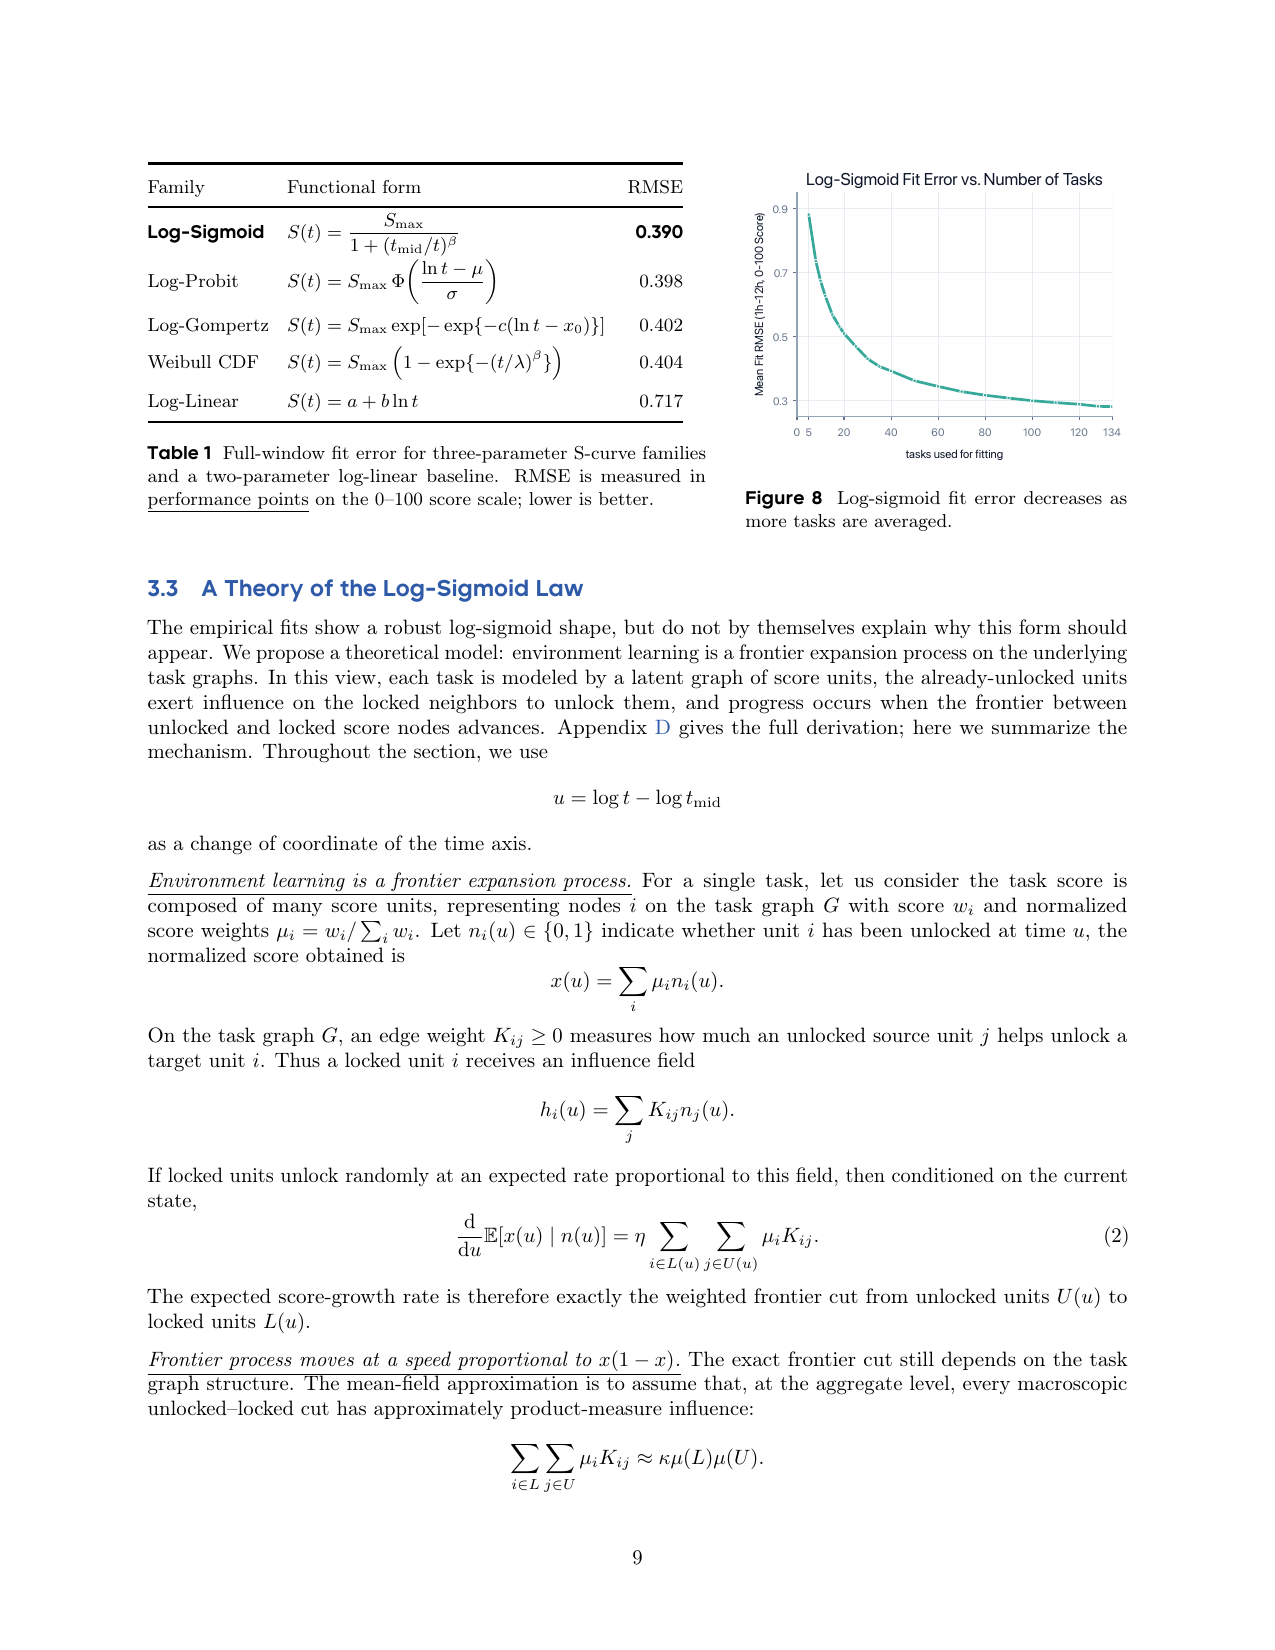
\includegraphics[width=0.95\textwidth]{figures/page-09.png}
\caption{对数-S 形拟合误差随求平均任务数的增加而降低。}
\label{fig:error-vs-tasks}
\end{figure}

% ============================================================
\subsection{对数-S 形规律的理论}
\label{sec:theory}

经验拟合展示出稳健的对数-S 形形状,但仅凭拟合本身并不能解释这一形状为何应该出现。我们提出一种理论模型:\textbf{环境学习是潜在任务图上的前沿扩张过程}。在这一视角下,每个任务被建模为一个``得分单元''的潜在图,已解锁的单元对锁定的邻居施加影响以解锁它们,当已解锁与已锁定得分节点之间的``前沿''推进时,进度即发生。附录~\ref{app:theory} 给出了完整推导,这里我们总结其机制。在本节中,我们使用 $u = \log t - \log t_{\mathrm{mid}}$ 作为时间轴的坐标变换。

\paragraph{环境学习是前沿扩张过程。} 对单一任务,设任务分数由许多得分单元构成,代表任务图 $G$ 上的节点 $i$,权重为 $w_{i}$,归一化得分权重为 $\mu_{i} = w_{i}/\sum_{i} w_{i}$。令 $n_{i}(u) \in \{0,1\}$ 指示单元 $i$ 在时间 $u$ 是否已解锁,则获得的归一化分数为:
\[
    x(u) = \sum_{i} \mu_{i}\,n_{i}(u).
\]
在任务图 $G$ 上,边权重 $K_{ij} \geq 0$ 度量已解锁源单元 $j$ 对解锁目标单元 $i$ 的帮助程度。因此,锁定的单元 $i$ 接收影响场:
\[
    h_{i}(u) = \sum_{j} K_{ij}\,n_{j}(u).
\]
若锁定单元以与该场成比例的期望速率\textbf{随机解锁},则在当前状态条件下:
\begin{equation}
    \frac{d}{du} \E[x(u) \mid n(u)] = \eta \sum_{i \in L(u)} \sum_{j \in U(u)} \mu_{i} K_{ij}.
    \label{eq:frontier}
\end{equation}
因此,期望分数增长率恰好等于从未解锁单元集 $U(u)$ 到锁定单元集 $L(u)$ 的\textbf{加权前沿切割}。

\paragraph{前沿过程以 $x(1-x)$ 的速度推进。} 精确的前沿切割仍依赖于任务图结构。均值场近似假设在聚合层面,每个宏观的``未解锁--锁定''切割都近似具有``乘积测度''的影响:
\[
    \sum_{i \in L}\sum_{j \in U} \mu_{i} K_{ij} \approx \kappa\, \mu(L)\,\mu(U),
\]
其中 $\mu(A) = \sum_{i \in A} \mu_{i}$。结合 \eqrefr{eq:frontier},得到:
\begin{equation}
    \frac{dx}{du} = \beta x(1-x), \qquad \beta = \eta \kappa.
    \label{eq:logistic}
\end{equation}
两个因子都有直接的物理解释:\textbf{已解锁的得分质量提供可复用能力},而\textbf{锁定的得分质量衡量剩余的改进机会}。附录~\ref{app:theory} 中的 D.2 节使用``加权切割混合''条件形式化了这一近似,该条件弱于``假设所有边权重各自相等''。

\paragraph{有效时间坐标是对数的。} 前沿方程写在有效的任务图坐标 $u$ 上。$u$ 近似 $\log t$ 的自然原因是\textbf{自相似图结构}\footnote{这让人联想到物理复杂系统中的自组织临界与临界现象——其行为不由单一特征尺度支配~\cite{bak1987self,newman2005power}。}。如果任务难度的每一\textbf{加法}增加暴露\textbf{乘法}更大的相关图结构,那么遍历图所需的搜索量随难度尺度\textbf{指数增长}。若跨时间尺度的搜索努力近似为常数,则时间 $t$ 所能达到的难度尺度满足:
\[
    u \sim \log t.
\]
将此坐标代入前沿方程 \eqrefr{eq:logistic} 即得:
\begin{equation}
    \frac{dx}{d\log t} = \beta x(1-x).
    \label{eq:logistic-log}
\end{equation}

\paragraph{求解前沿方程。} 分离变量于 \eqrefr{eq:logistic-log} 得:
\[
    \log \frac{x(t)}{1 - x(t)} = \beta \log \frac{t}{t_{\mathrm{mid}}},
\]
其中 $t_{\mathrm{mid}}$ 选取使得 $x(t_{\mathrm{mid}}) = 1/2$。因此:
\begin{equation}
    \frac{1}{S_{\max}} = \frac{1}{1 + (t_{\mathrm{mid}}/t)^{\beta}} \quad\Longrightarrow\quad S(t) = \frac{S_{\max}}{1 + (t_{\mathrm{mid}}/t)^{\beta}}.
    \label{eq:solve}
\end{equation}
即重新得到式~\ref{eq:log-sigmoid}。

\paragraph{基准均值比单个任务更平滑。} 上面的论证刻画的是\textbf{极限前沿漂移}。它\textbf{并不意味着}每个有限任务都会以肉眼可见的平滑 S 形推进。仅有少量得分单元的任务可能呈现长平台与突然跳跃。经验缩放规律是关于\textbf{任务聚合曲线}的命题:若许多独立评测的任务各自遵循近似的前沿动力学,则求平均会消除有限任务的锯齿状。当残余任务中点与任务速度足够集中时,聚合曲线将退化为单一对数-S 形:
\[
    \frac{1}{M}\sum_{b=1}^{M} x_{b}(u) \approx \frac{1}{M}\sum_{b=1}^{M} \frac{1}{1 + e^{-\beta(u - \delta_{b})}} \xrightarrow{P} \frac{1}{1 + e^{-\beta u}}.
\]
附录~\ref{app:theory} 中的 D.3 节在``逐块切割混合''、``跳跃噪声平均消失''、``中点对齐''与``速度集中''等假设下给出了精确表述。

\paragraph{拟合参数的解读。} 拟合速率 $\beta$ 可自然地解读为对数时间下的\textbf{有效前沿传播速度}。较大的 $\beta$ 意味着分数解锁发生在更窄的交互尺度区间内,产生由低到高的更陡跃迁;较小的 $\beta$ 意味着进度分散于更多的乘法时间上,产生更平缓的学习曲线。拟合上限 $S_{\max}$ 应解读为\textit{拟合区间}内\textbf{可达的分数支撑},而非性能绝对意义上的\textbf{上界}。

\paragraph{适用范围与局限。} 对数-S 形规律并非对每个环境学习过程都成立。当任务图含有强瓶颈、分散的任务中点、异构的前沿速度或非自相似图结构时,该规律可能失效。这些失败模式澄清了理论的范围:对数-S 形在``进度表现为在近似分形结构图上充分混合的前沿扩张过程''时最自然。在此意义上,从环境中学习衡量的是智能体能否\textbf{将多样化反馈转化为可复用的结构},从而加速后续发现。我们认为这是``环境学习值得度量与扩展''的核心原因。

% ============================================================
\section{智能体学习速度大约每三个月翻倍}
\label{sec:speed}

前沿智能体现在能够通过与任务环境的交互来提升表现。这引出一个独立问题:较新的模型是否学习得更快?我们通过比较各智能体在\textbf{固定交互预算}下获得的性能增益,按模型发布日期衡量。

\subsection{实验设计}
\label{sec:speed-design}

\paragraph{分离先验知识与环境学习。} 高分可能反映模型已经掌握的知识,而非在运行中学到的内容。为减少这一混淆,我们从 EdgeBench 中选取一个 18 任务的子集,这些任务上模型表现出相近的首次尝试性能。由于起点相当,后续增益提供了对环境学习的更纯净度量。我们将``任务学习速度''定义为\textbf{在固定两小时预算下的平均性能增益}。

\paragraph{评测协议。} 我们评测自 2025 年 9 月(前沿系统开始具备持续自主运行能力时)至当前评测窗口期间发布的前沿开源与闭源 AI 系统。每个模型每个任务运行三次。GPT 系列模型使用 Codex 运行;所有其他模型使用 Claude Code 运行。如 \figref{fig:initial-vs-best} 左图所示,模型在该 18 任务子集上从可比的首次尝试性能起步,平均 $6.87 \pm 0.97$。

\subsection{跨模型代际的学习速度}

\figref{fig:speed-trend} 报告了在固定 18 任务子集上的两小时评测结果。纵轴以对数尺度衡量智能体学习速度,定义为两小时内的性能增益。为估计前沿趋势,我们以深色标记突出每个发布日的\textbf{前两名}模型,然后对这些前沿点拟合线性趋势,95\% 置信区间显示为阴影带。

\figref{fig:speed-trend} 显示了近期模型代际间学习速度的快速提升。从 2025 年 9 月的 GPT-5-Codex 到 2026 年 4 月的 GPT-5.5,学习速度在 221 天内增长约 \textbf{8 倍}。对前沿模型的对数-线性拟合很好地捕捉了这一趋势,对应于\textbf{大约每三个月翻一倍}。\figref{fig:initial-vs-best} 显示该改进并不能简单地用``更频繁提交''解释。提交频率(右图)变化不均匀:较新的 GPT 模型提交更频繁,而其他家族则不然。中图讲述了一个不同的故事:较新的模型能将\textbf{更大比例}的提交转化为``迄今最佳''改进。因此,该趋势反映的是每次交互中\textbf{更有效的学习},而不仅仅是更多尝试。

\begin{figure}[h]
\centering
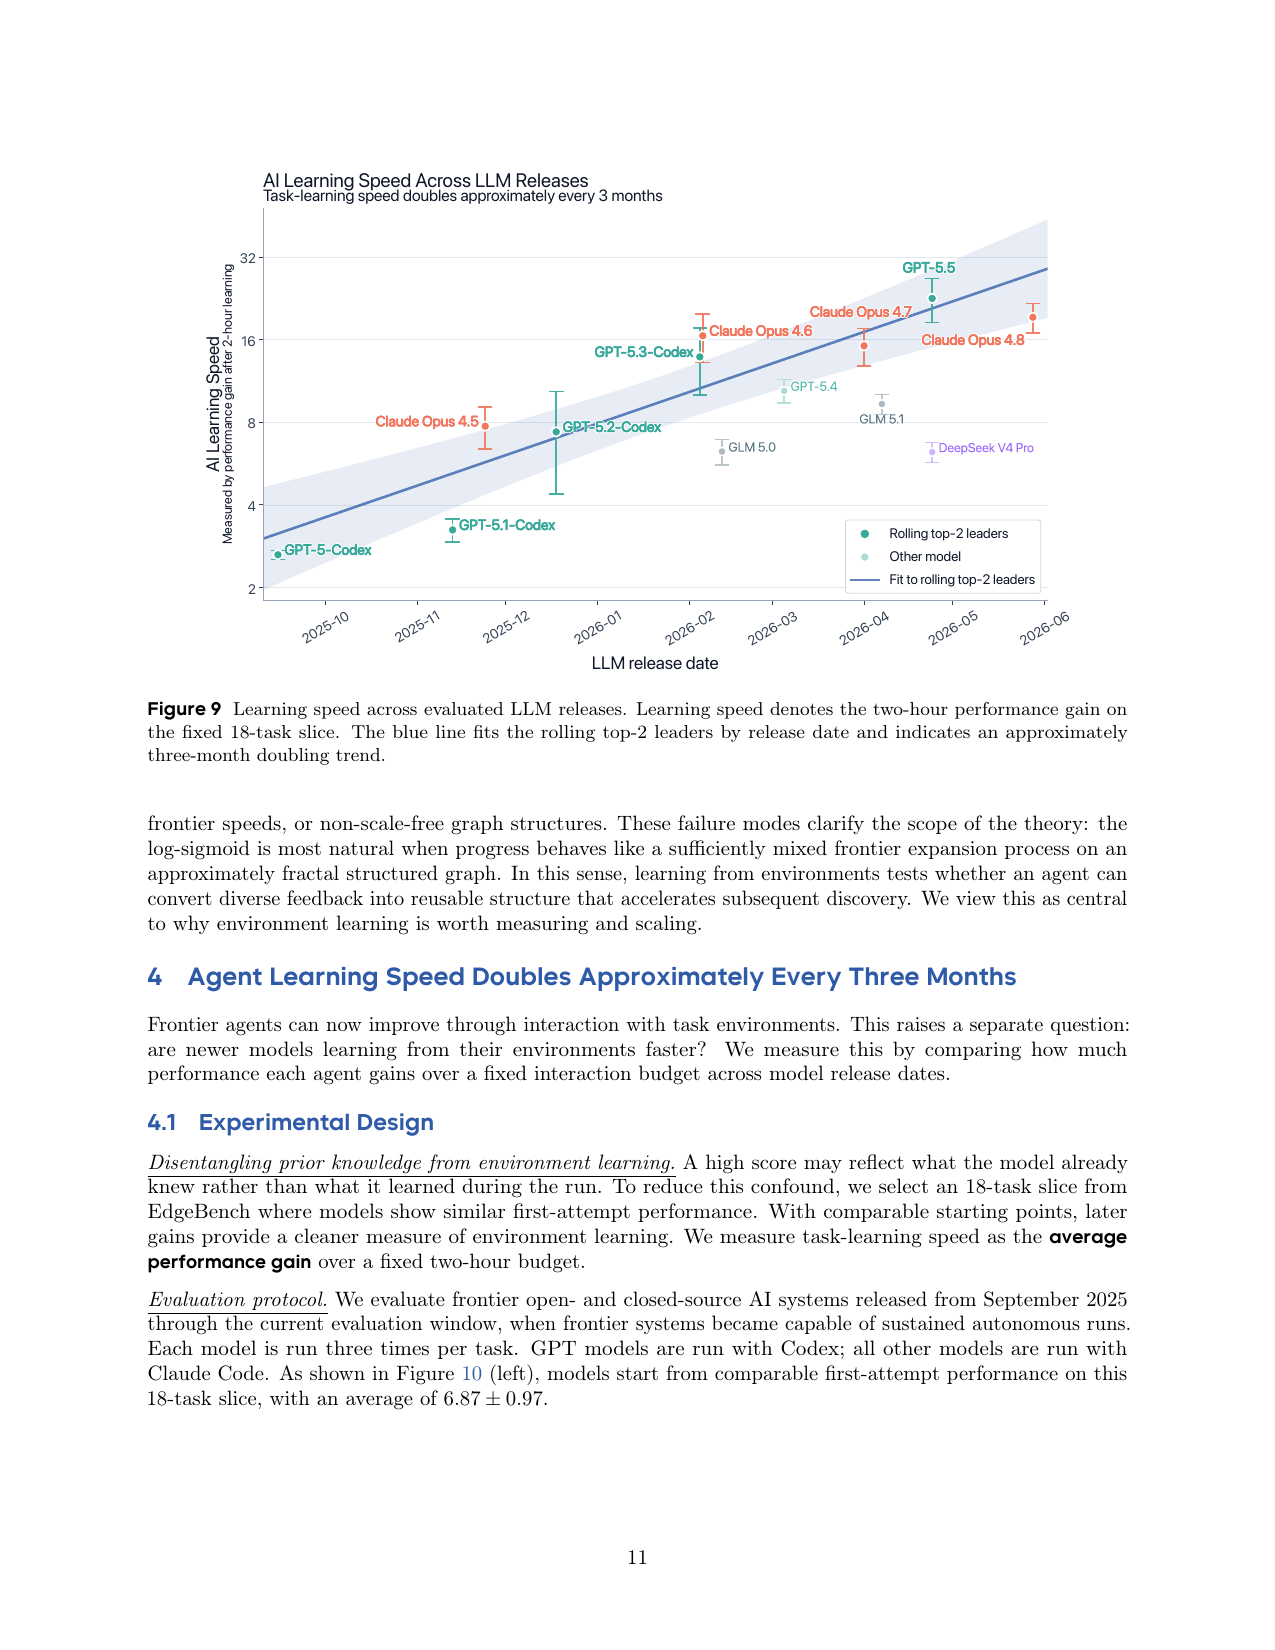
\includegraphics[width=0.95\textwidth]{figures/page-11.png}
\caption{跨 LLM 发布日 AI 学习速度的演进。学习速度定义为固定 18 任务子集上的两小时性能增益。蓝色线对发布日的滚动前两名进行拟合,显示大约三个月翻倍的趋势。}
\label{fig:speed-trend}
\end{figure}

\begin{figure}[h]
\centering
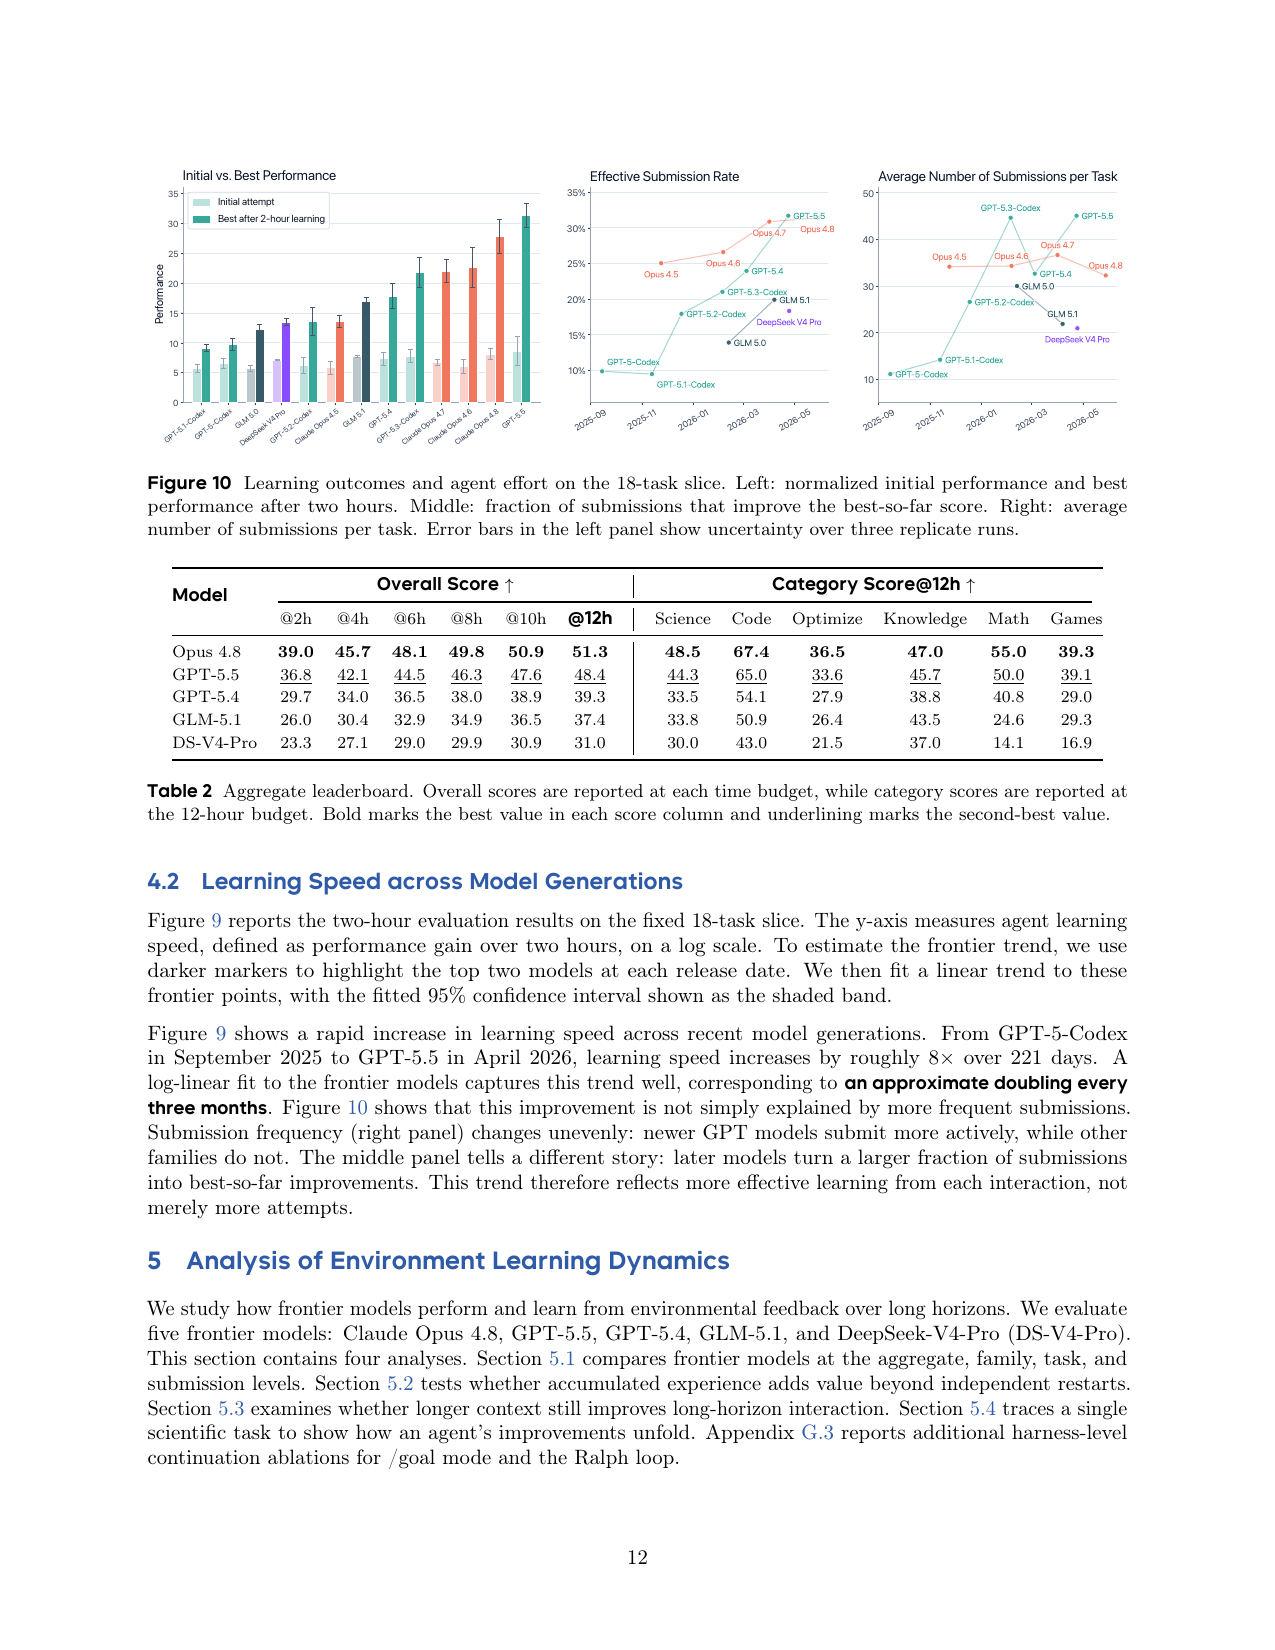
\includegraphics[width=0.95\textwidth]{figures/page-12.png}
\caption{18 任务子集上的学习结果与智能体投入。左:归一化初始性能与两小时学习后的最佳性能。中:改进``迄今最佳''分数的提交比例。右:每个任务的平均提交次数。左图误差棒显示三次重复运行的不确定性。}
\label{fig:initial-vs-best}
\end{figure}

\begin{table}[h]
\centering
\small
\setlength{\tabcolsep}{4pt}
\begin{tabular}{l cccccc c cccccc}
\toprule
\multirow{2}{*}{\textbf{模型}} & \multicolumn{6}{c}{\textbf{总分 $\uparrow$}} & & \multicolumn{6}{c}{\textbf{12 小时分家族分数 $\uparrow$}} \\
\cmidrule(lr){2-7} \cmidrule(lr){9-14}
 & @2h & @4h & @6h & @8h & @10h & @12h & & 科学 & 代码 & 优化 & 知识 & 数学 & 游戏 \\
\midrule
Opus 4.8 & 39.0 & 45.7 & 48.1 & 49.8 & 50.9 & \textbf{51.3} & & 48.5 & \textbf{67.4} & 36.5 & \textbf{47.0} & \textbf{55.0} & \textbf{39.3} \\
GPT-5.5 & 36.8 & 42.1 & 44.5 & 46.3 & 47.6 & \underline{48.4} & & 44.3 & 65.0 & 33.6 & 45.7 & 50.0 & 39.1 \\
GPT-5.4 & 29.7 & 34.0 & 36.5 & 38.0 & 38.9 & 39.3 & & \underline{33.5} & 54.1 & 27.9 & 38.8 & 40.8 & 29.0 \\
GLM-5.1 & 26.0 & 30.4 & 32.9 & 34.9 & 36.5 & 37.4 & & 33.8 & 50.9 & \underline{26.4} & \underline{43.5} & 24.6 & 29.3 \\
DS-V4-Pro & 23.3 & 27.1 & 29.0 & 29.9 & 30.9 & 31.0 & & 30.0 & 43.0 & 21.5 & 37.0 & 14.1 & 16.9 \\
\bottomrule
\end{tabular}
\caption{聚合排行榜。总分报告于每个时间预算;分家族分数报告于 12 小时预算。\textbf{加粗}为该列最佳值,\underline{下划线}为次佳。}
\label{tab:leaderboard}
\end{table}

% ============================================================
\section{环境学习动力学分析}
\label{sec:dynamics}

我们研究前沿模型如何在长视野下利用环境反馈进行表现与学习。我们评测五个前沿模型:Claude Opus 4.8、GPT-5.5、GPT-5.4、GLM-5.1 与 DeepSeek-V4-Pro(DS-V4-Pro)。本节包含四项分析。\secref{sec:model-compare} 从聚合、家族、任务与提交层面比较前沿模型;\secref{sec:experience} 测试累积经验是否相比独立重启具有额外价值;\secref{sec:ctx} 检验更长上下文是否在长视野交互中提升性能;\secref{sec:case-study} 跟踪一个科学任务以展示智能体改进的具体展开方式。附录~\ref{app:harness} 报告了 ``/goal 模式'' 与 ``Ralph 循环'' 在沙箱级别的额外续接消融。

\subsection{前沿模型比较}
\label{sec:model-compare}

\paragraph{设置。} 我们沿用 \secref{sec:exp-setup} 的设置,并从两个角度分析 12 小时轨迹:(1) 聚合、家族与任务层面的表现;以及 (2) 提交效率,即智能体的提交有多频繁地改进当前最佳。

\paragraph{表现比较。} 表~\ref{tab:leaderboard} 给出聚合表现。Claude Opus 4.8 在 12 小时达到 \textbf{51.3} 分,其次是 GPT-5.5 的 \textbf{48.4}。GPT-5.4 与 GLM-5.1 组成下一梯队(39.3 与 37.4),DS-V4-Pro 取得 31.0。家族级结果与聚合排名大体一致:Claude Opus 4.8 在每个家族均值上领先,GPT-5.5 在游戏上尤其接近且总体排名第二。详细逐任务表现见附录~\ref{app:score-tables},$\ast$ 标记少于三次有效运行的单元格。

\begin{figure}[h]
\centering
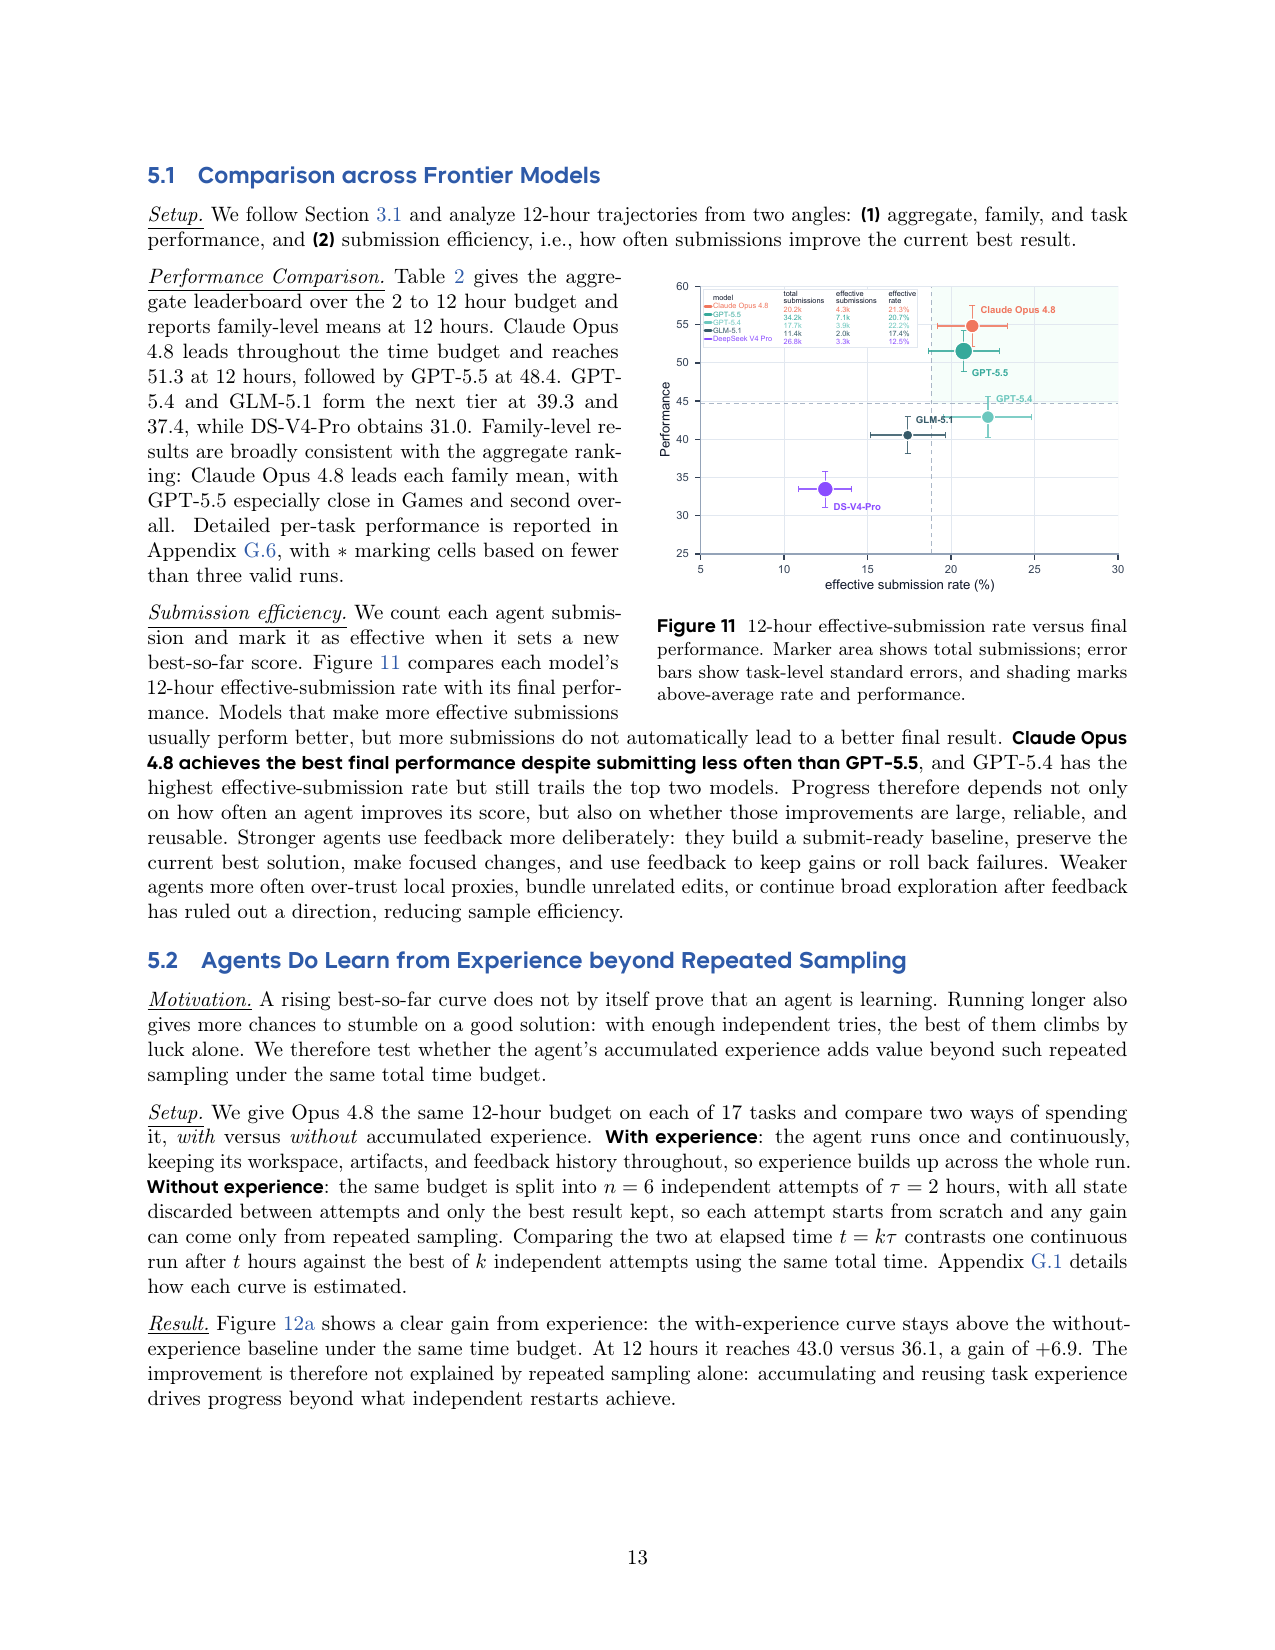
\includegraphics[width=0.95\textwidth]{figures/page-13.png}
\caption{12 小时有效提交率与最终表现的对比。标记面积表示总提交数;误差棒表示任务级标准误;阴影标记高于均值水平。}
\label{fig:submission-vs-perf}
\end{figure}

\paragraph{提交效率。} 我们对每个智能体的每次提交计数,当其将``迄今最佳''分数推至新高时标记为``有效''。\figref{fig:submission-vs-perf} 比较了各模型 12 小时的有效提交率与最终表现。做出更多有效提交的模型通常表现更好,但``更多提交''并不自动带来更好的最终结果。\textbf{Claude Opus 4.8} 取得了最佳最终表现,即便其提交频率低于 GPT-5.5;GPT-5.4 拥有最高有效提交率,但仍落后于前两名。因此,进度不仅取决于智能体改进分数的频率,还取决于改进是否\textbf{大、可靠且可复用}。较强的智能体会更审慎地使用反馈:构建可提交的基线、保留当前最佳方案、做出有针对性的改动,并利用反馈保留收益或回滚失败。较弱的智能体则更倾向于\textbf{过度信任本地代理、捆绑无关修改或在反馈已排除某方向后仍继续广泛探索},从而降低采样效率。

\subsection{智能体确实从经验中学习,而非仅仅重复采样}
\label{sec:experience}

\paragraph{动机。} ``迄今最佳''曲线不断上升本身并不能证明智能体在``学习''。运行更长时间同样增加偶然撞到好解的机会:在足够多的独立尝试下,最佳的尝试仅凭运气就能提升。因此,我们测试智能体的\textbf{累积经验}是否在相同总时间预算下,比单纯重复采样带来额外价值。

\paragraph{设置。} 我们在 17 个任务上为 Opus 4.8 给出相同的 12 小时预算,并比较两种花费方式:\textbf{有经验} vs.\ \textbf{无经验}。
\begin{itemize}
    \item \textbf{有经验}:智能体连续运行一次,保留其工作区、产物与反馈历史,使经验跨整个运行积累。
    \item \textbf{无经验}:同样预算被切分为 $n = 6$ 次独立的 $\tau = 2$ 小时尝试,各次之间丢弃所有状态,只保留最佳结果,因此每次尝试从头开始,任何增益只能来自重复采样。
\end{itemize}
在经过时间 $t = k\tau$ 时,二者对比即``一次连续运行 $t$ 小时后''与``使用相同总时间的 $k$ 次独立尝试中最佳者''。附录~\ref{app:exp-curves} 详细描述了如何估计各曲线。

\paragraph{结果。} \figref{fig:exp-vs-no-exp} 显示经验带来明显收益:在相同时间预算下,``有经验''曲线始终高于``无经验''基线。在 12 小时,其达到 43.0 vs.\ 36.1,提升 $+6.9$。因此,该改进\textbf{不能}单独由重复采样解释:累积并复用任务经验驱动了独立重启所无法达到的进度。

\begin{figure}[h]
\centering
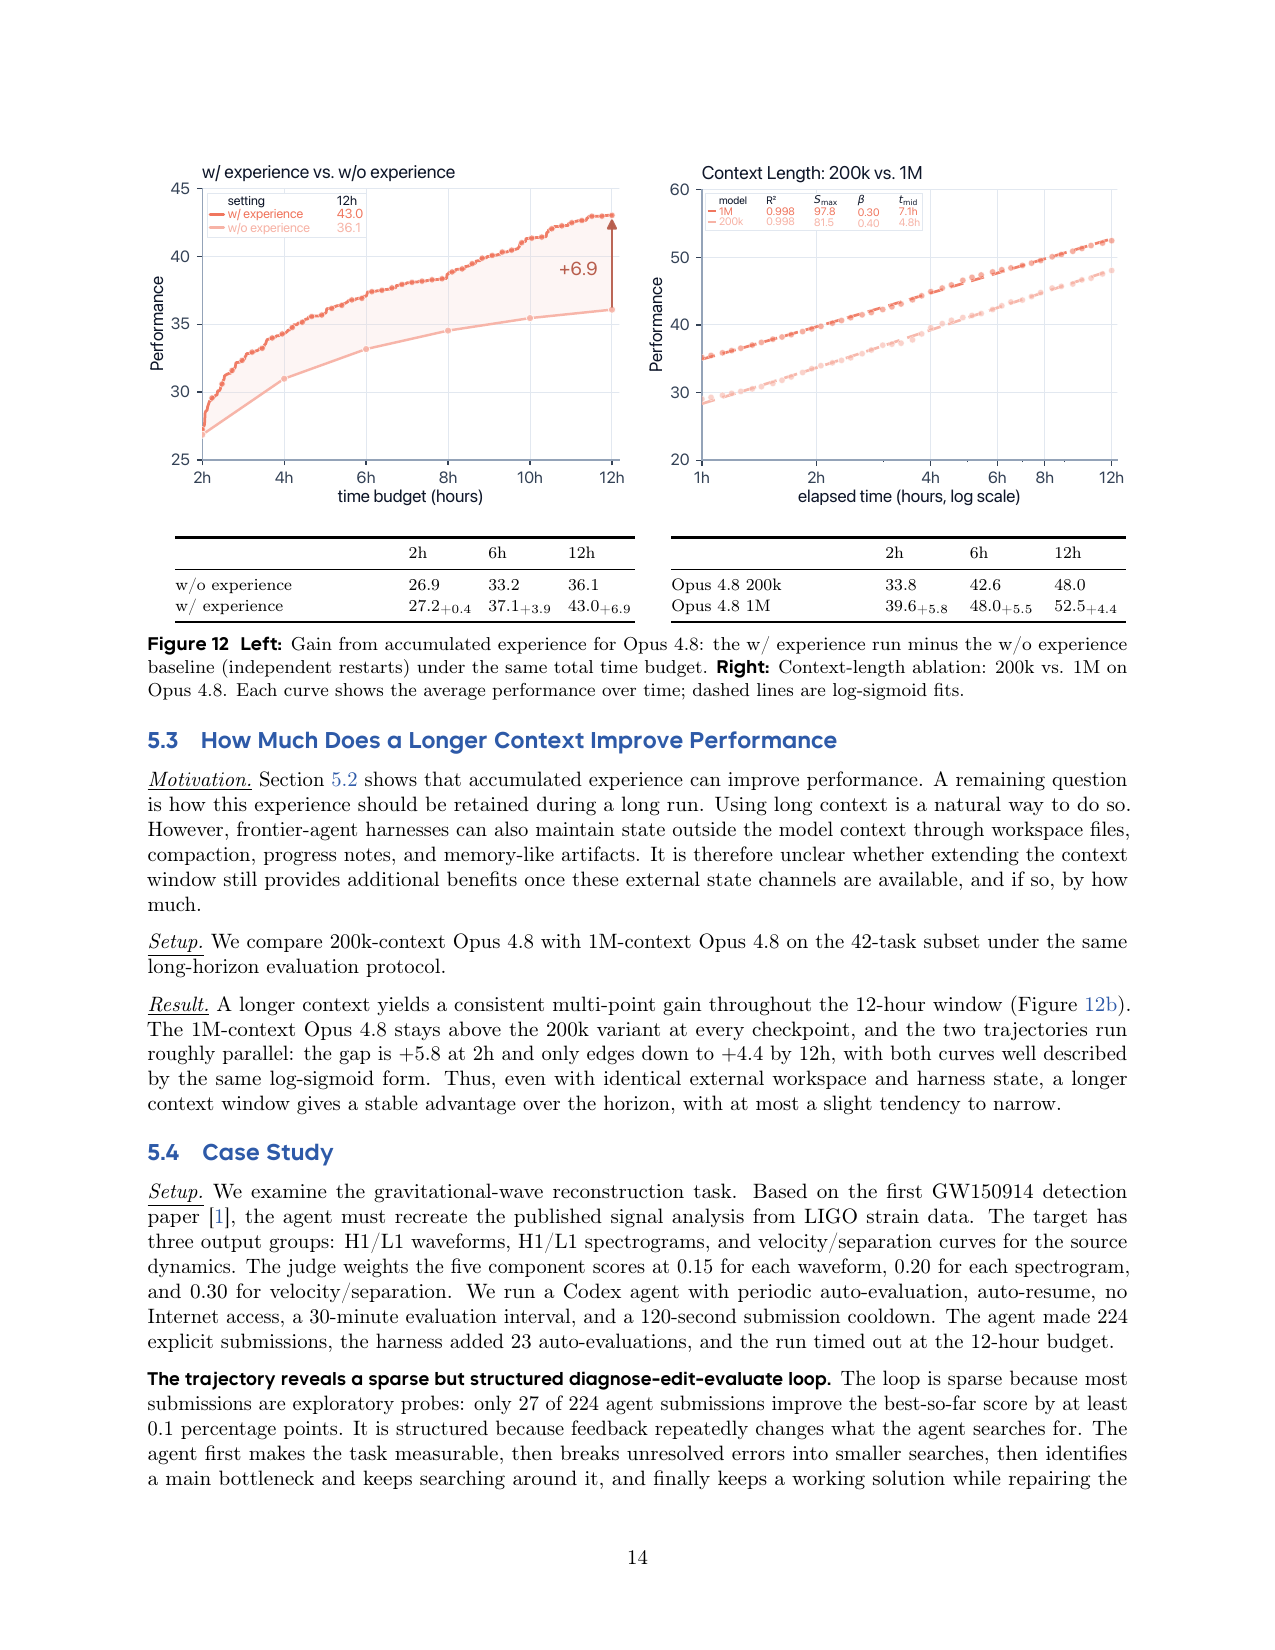
\includegraphics[width=0.95\textwidth]{figures/page-14.png}
\caption{左:Opus 4.8 在相同总时间预算下``有经验''减去``无经验''(独立重启)的增益。右:上下文长度消融,200k 与 1M 在 Opus 4.8 上的对比。每条曲线显示平均性能随时间变化;虚线为对数-S 形拟合。}
\label{fig:exp-vs-no-exp}
\end{figure}

\subsection{更长上下文对性能有多少提升?}
\label{sec:ctx}

\paragraph{动机。} \secref{sec:experience} 表明累积经验能提升性能。一个悬而未决的问题是,在长运行中应当如何保留经验。使用长上下文是一种自然的方法。然而,前沿智能体框架也可通过工作区文件、压缩、进度备忘以及类记忆制品,在模型上下文之外维护状态。因此,在这些外部状态通道已可用的情况下,扩展上下文窗口是否仍能带来额外收益(若有,多大)并不明确。

\paragraph{设置。} 我们在 42 任务子集上,在相同的长视野评测协议下比较 200k 上下文的 Opus 4.8 与 1M 上下文的 Opus 4.8。

\paragraph{结果。} 更长的上下文在整个 12 小时窗口上带来稳定的多点提升(\figref{fig:exp-vs-no-exp} 右)。1M 上下文的 Opus 4.8 在每个检查点上都高于 200k 版本,两条轨迹近乎平行:差距在 2h 时为 $+5.8$,到 12h 仅略微收窄到 $+4.4$,且两条曲线均很好地符合相同的对数-S 形形式。因此,即便具有相同的工作区与沙箱状态,更长的上下文窗口在整段视野上都提供了稳定优势,且仅有略微收窄的趋势。

\subsection{案例研究}
\label{sec:case-study}

\paragraph{设置。} 我们考察\textbf{引力波重构}任务。基于首篇 GW150914 检测论文~\cite{abbott2016gw150914},智能体需要从 LIGO 应变数据复现已发表的信号分析。目标分三组输出:H1/L1 波形、H1/L1 时频谱、以及源动力学(速度/分离度)曲线。判官权重将五个组件分数设为:每个波形 0.15,每个时频谱 0.20,以及速度/分离 0.30。我们以 30 分钟评测间隔与 120 秒提交冷却运行 Codex 智能体,并禁用网络访问。智能体进行了 224 次显式提交,沙箱增加了 23 次自动评测,运行在 12 小时预算时超时。

\paragraph{轨迹揭示了稀疏但结构化的``诊断--编辑--评测''循环。} 该循环之所以稀疏,是因为大部分提交是探索性试探:只有 224 次智能体提交中的 27 次将``迄今最佳''分数提升至少 0.1 个百分点。其结构性在于反馈反复改变了智能体的搜索方向:智能体首先使任务\textbf{可度量},然后将未解决的错误拆分为更小的搜索,识别主要瓶颈并持续围绕其搜索,最后保留一个可行方案同时修复剩余错误。这些模式展示了``许多失败的试探仍能产出少量累积改进''。

\begin{figure}[h]
\centering
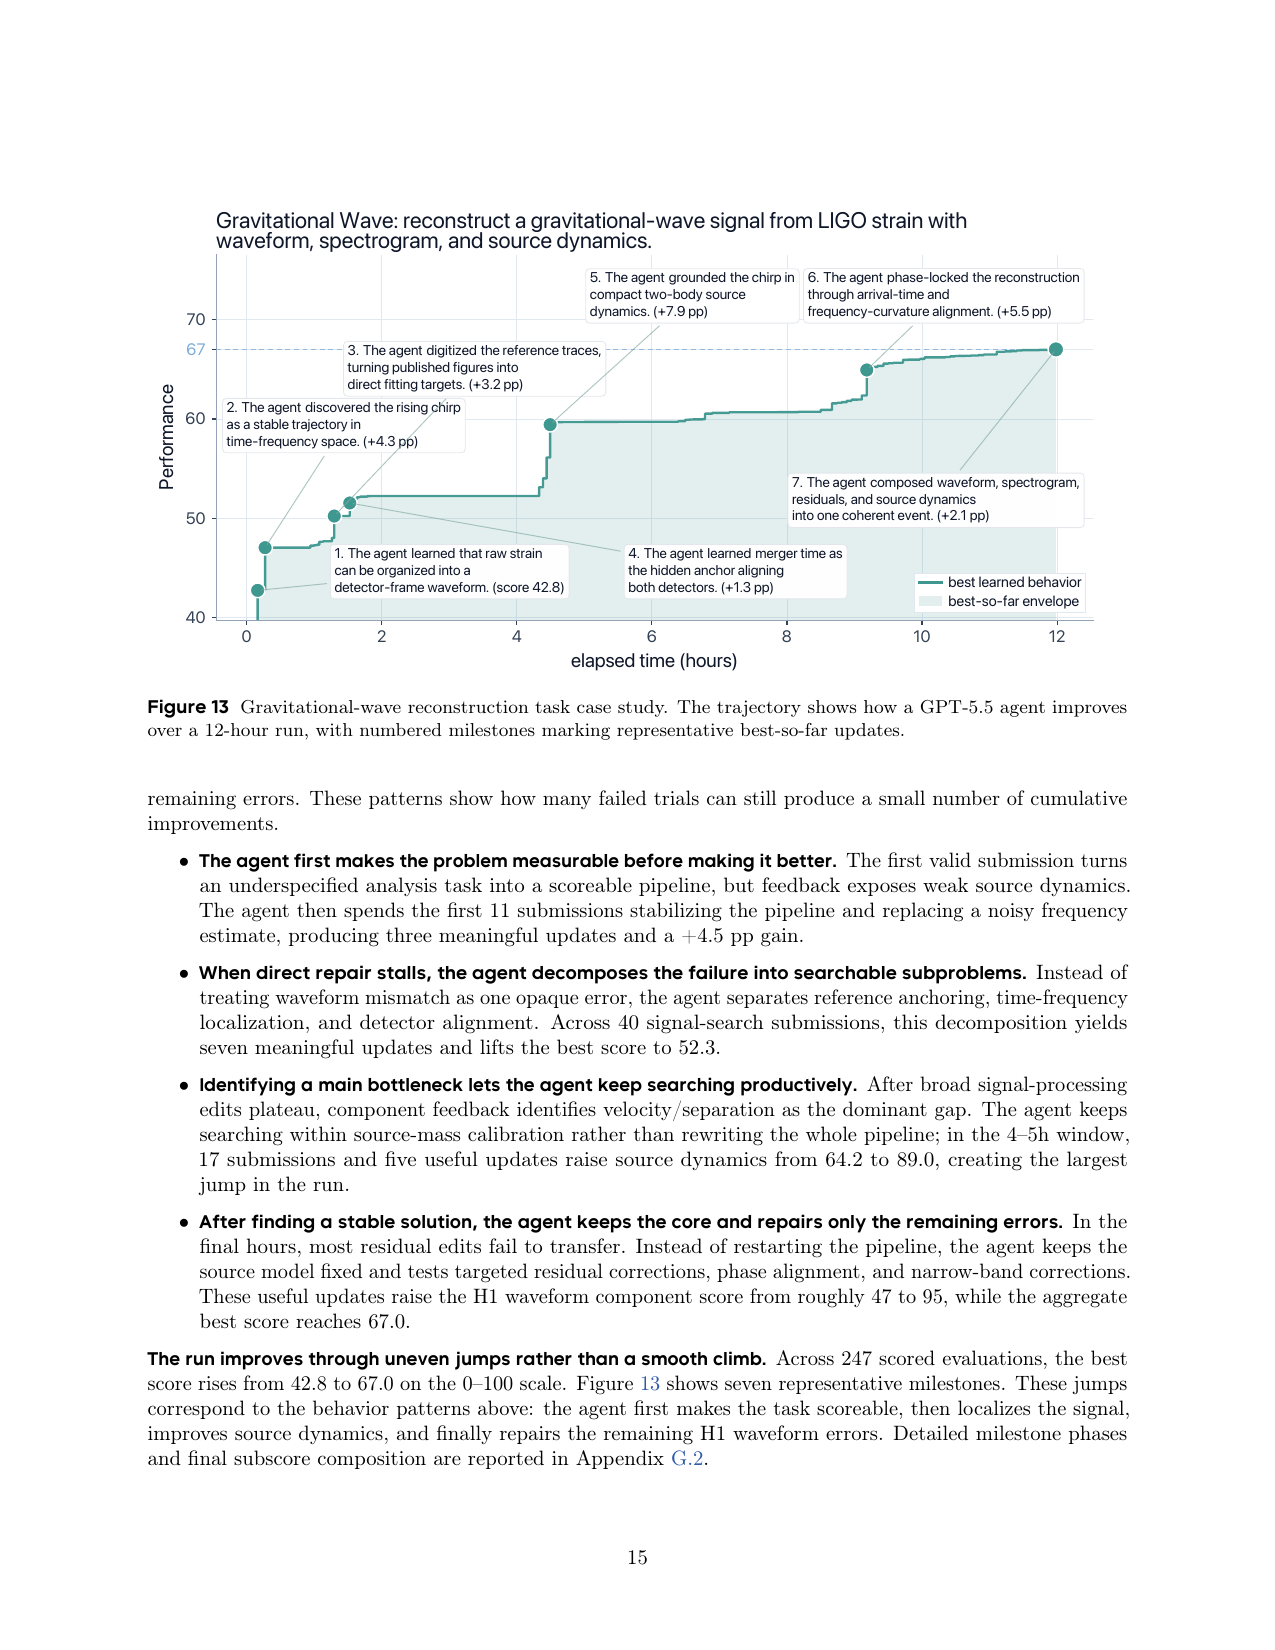
\includegraphics[width=0.95\textwidth]{figures/page-15.png}
\caption{引力波重构任务案例研究。该轨迹展示了 GPT-5.5 智能体如何在 12 小时运行中改进;编号里程碑标记代表性的最佳更新。任务说明:从 LIGO 应变重构引力波信号,包含波形、时频谱与源动力学。}
\label{fig:case-study}
\end{figure}

\paragraph{详细阶段:}
\begin{itemize}
    \item \textbf{智能体首先使问题可度量,然后再使其更好。} 第一次有效提交将一项定义不清的分析任务转换为可打分的流水线,但反馈暴露了薄弱的源动力学。随后智能体在最初 11 次提交中稳定该流水线并替换一个噪声较大的频率估计,产生三次有意义的更新与 $+4.5$ 个百分点的提升。
    \item \textbf{直接修复停滞时,智能体将失败分解为可搜索的子问题。} 智能体并未将波形不匹配视为一个不透明错误,而是将参考锚定、时频定位与探测器对齐分离开来。在 40 次信号搜索提交中,这种分解产生七次有意义的更新,将最佳分数提升至 52.3。
    \item \textbf{识别主要瓶颈使智能体持续高效搜索。} 在广义信号处理编辑进入平台期后,组件反馈将``速度/分离''识别为最显著差距。智能体在源质量校准内继续搜索,而非重写整条流水线;在 4--5 小时窗口中,17 次提交与 5 次有效更新将源动力学从 64.2 提升至 89.0,造成整个运行中最大的跳跃。
    \item \textbf{找到稳定方案后,智能体保留核心并仅修复剩余错误。} 在最后几小时,大多数残差编辑无法迁移。智能体保留源模型固定,转而测试有针对性的残差校正、相位对齐与窄带校正。这些有效更新将 H1 波形组件分数从约 47 提升至 95,聚合最佳分达到 67.0。
\end{itemize}

\paragraph{通过不均匀跳跃而非平滑爬升实现改进。} 在 247 次打分评测中,最佳分数在 0--100 分制上从 42.8 升至 67.0。\figref{fig:case-study} 展示了 7 个代表性里程碑。这些跳跃对应上述行为模式:智能体首先使任务可打分,接着定位信号、改进源动力学,最后修复剩余的 H1 波形错误。详细里程碑阶段与最终子分构成见附录~\ref{app:case-study}。

% ============================================================
\section{相关工作}
\label{sec:related}

\begin{table}[h]
\centering
\small
\setlength{\tabcolsep}{4pt}
\begin{tabular}{lcccl}
\toprule
\textbf{基准} & \textbf{\#任务} & \textbf{视野} & \textbf{场景} & \textbf{自演化} \\
\midrule
MMLU~\cite{hendrycks2021mmlu} & 15{,}908 & 短 & 知识问答 & 否 \\
AIME~\cite{maa2026aime} & 30 & 短 & 高中数学竞赛 & 否 \\
GDPval Gold~\cite{patwardhan2025gdpval} & 220 & 短 & 专业交付物 & 否 \\
SWE-bench Verified~\cite{jimenez2024swebench,openai2024swebench} & 500 & 短 & Issue 修复 & 否 \\
Terminal-Bench 2.0~\cite{merrill2026terminalbench} & 89 & 短 & 终端工作流 & 否 \\
Continual Learning Bench~\cite{asawa2026clbench} & 6 & 短 & 受控任务序列 & 是 \\
CL-bench~\cite{dou2026clbench} & 1{,}899 & 短 & 上下文学习 & 否 \\
FrontierCode~\cite{lu2026frontiercode} & 150 & N/A & 生产代码改动 & 否 \\
NL2Repo-Bench~\cite{ding2025nl2repo} & 104 & 中 & 仓库生成 & 否 \\
Agents' Last Exam~\cite{sun2026agents} & 152 (公开) & 中 & 计算机使用工作流 & 否 \\
MLE-bench~\cite{chan2025mle} & 75 & 长 & ML 工程 & 是 \\
MLS-Bench~\cite{lyu2026mlsbench} & 140 & 长 & ML 研究 & 子集 \\
Frontier-Eng~\cite{chi2026frontiereng} & 47 & 长 & 工程设计 & 否 \\
Frontier-CS~\cite{mang2025frontiercs} & 156 & 长 & 开放式 CS 任务 & 否 \\
AutoLab~\cite{xu2026autolab} & 36 & 长 & 研究/工程优化 & 否 \\
FrontierSWE~\cite{chu2026frontierswe} & 17 & 长 & 软件工程/性能调优 & 否 \\
\textbf{EdgeBench(本文)} & \textbf{134} & \textbf{超长} & \textbf{软件工程, 科学/ML, 专业工作, 优化, 形式化证明, 游戏} & \textbf{是} \\
\bottomrule
\end{tabular}
\caption{与代表性基准的比较。``视野''刻画的是单实例任务合约,非套件总运行时间。仅当性能被显式地相对于资源轴(如时间或样本数)绘制时,才计为``自演化''。}
\label{tab:bench-compare}
\end{table}

\paragraph{现有基准覆盖了智能体能力的大部分,但很少衡量智能体如何在一次运行内改进。} 闭卷问答、数学与编程基准(如 MMLU~\cite{hendrycks2021mmlu}、AIME~\cite{maa2026aime}、HumanEval~\cite{chen2021humaneval})以及端点补丁基准(如 SWE-bench~\cite{jimenez2024swebench})评估的是最终答案或最终补丁。更多的智能体与面向工作的基准,包括 GDPval~\cite{patwardhan2025gdpval}、Agents' Last Exam~\cite{sun2026agents} 和 FrontierCode~\cite{lu2026frontiercode},将任务接口扩展到专业交付物、计算机使用工作流或生产代码改动。然而,其报告的中心指标仍是端点度量:任务成功率、产物质量、通过率或生产就绪度。EdgeBench 转而衡量\textbf{随时间改进的轨迹}。

\paragraph{某些基准研究学习,但聚焦于受限领域与较短视野。} CL-bench~\cite{dou2026clbench}、EvaLearn~\cite{dou2025evalearn} 和 Continual Learning Bench~\cite{asawa2026clbench} 评估模型能否从\textbf{静态上下文}或\textbf{静态信息流}中改进——其内容主要并非由智能体在单任务内的行为塑造。迭代优化基准,如 MLE-bench~\cite{chan2025mle}、MLS-Bench~\cite{lyu2026mlsbench}、Frontier-Eng~\cite{chi2026frontiereng}、Frontier-CS~\cite{mang2025frontiercs} 与 ALE-Bench~\cite{imajuku2025alebench},进一步纳入了重复尝试、经验反馈或可见的指标。最接近的长视野智能体对比基准是 AutoLab~\cite{xu2026autolab} 与 FrontierSWE~\cite{chu2026frontierswe}:两者均评估能反复编辑可执行产物并吸收反馈的智能体。EdgeBench 的差异在于覆盖了更广泛的可执行领域、采用日级任务合约,并在所有任务上一致地应用相同的轨迹度量。

\paragraph{缩放规律在先前工作中已被广泛研究,但从多样化真实环境中学习仍未被充分探索。} 经典缩放规律研究预训练,将损失或基准性能与模型规模、数据与算力联系起来~\cite{kaplan2020,hoffmann2022};后续工作研究了模型规模扩展下有界基准性能曲线~\cite{bhagia2024ladder,owen2024predictable,ruan2024observational,zhang2026prescriptive}。测试时缩放规律也已在多种推理时方法下被研究:纯重复采样~\cite{chen2021humaneval,li2022alphacode,brown2024monkeys}、搜索、修订或验证器引导的计算分配~\cite{snell2024scalingllm,wunips2024inference},以及推理模型中的长链思维推理~\cite{openaio1,deepseek2025r1}。智能体测试时缩放已在计算机使用与浏览智能体中被观察到~\cite{openai2025cua,wei2025browsecomp},通过交互长度缩放开展研究~\cite{shen2025thinkingvsdoing},并经由长视野人-智能体比较被重新审视~\cite{mang2026humansdontjustsample}。这些研究更接近我们的设置,但覆盖的领域更窄、任务更少,且未建立跨域的缩放规律。强化学习缩放也与之相关,因为它研究从环境反馈中学习~\cite{hilton2023scalingrl,khatri2025rlart};而 EdgeBench 测量的是已部署智能体轨迹中的\textit{已用交互时间}。从任务反馈中做上下文学习(In-Context Learning, ICL) 相对廉价,可跨许多可执行环境反复评测;而大规模强化学习运行代价高昂,通常覆盖环境较少。EdgeBench 更广的环境覆盖或许正是聚合曲线稳定到足以揭示缩放规律的原因。

更详细的逐基准讨论见附录~\ref{app:related}。

% ============================================================
\section{结论}
\label{sec:conclusion}

本文介绍了 EdgeBench——一个用于研究智能体如何在\textbf{日级视野}下从真实世界环境中学习的基准。在 134 个多样化可执行任务与约 38{,}000 小时的环境交互上,我们发现聚合学习轨迹遵循与交互时间的精确\textbf{对数-S 形关系}。同一形式跨任务家族保持稳定,在更长视野下保持稳定,并支持从早期轨迹预测后期性能。我们还发现智能体的\textbf{学习速度}在近期前沿模型代际间快速提升。

这些结果表明,从环境中学习并非一系列零散的任务结果,而是\textbf{可度量的缩放对象}。与许多聚合能力曲线不同,环境学习轨迹揭示了产生进步的中间尝试、反馈与修订。这使得 EdgeBench 不仅可用于为智能体排名,还可用于研究智能体如何获得并复用经验。

更广泛地说,我们观察到的规律性表明:部署后从丰富环境中学习或许值得享有与预训练相同的\textbf{系统性缩放关注}。
